%% ----------------------------------------------------------------
%% Thesis.tex -- MAIN FILE (the one that you compile with LaTeX)
%% ---------------------------------------------------------------- 

% Set up the document
\documentclass[a4paper, 12pt, twoside]{Thesis}  % Use the "Thesis" style, based on the ECS Thesis style by Steve Gunn
% \documentclass[a4paper, 12pt, oneside]{Thesis}  % Use the "Thesis" style, based on the ECS Thesis style by Steve Gunn
\graphicspath{{Figures/}}  % Location of the graphics files (set up for graphics to be in PDF format)

% Include any extra LaTeX packages required
\usepackage{verbatim}  % Needed for the "comment" environment to make LaTeX comments
\hypersetup{urlcolor=blue, colorlinks=true}  % Colours hyperlinks in blue, but this can be distracting if there are many links.

%% ----------------------------------------------------------------
\begin{document}
\frontmatter	  % Begin Roman style (i, ii, iii, iv...) page numbering

\maketitle
\makesecondtitle
%% ----------------------------------------------------------------

\setstretch{1.3}  % It is better to have smaller font and larger line spacing than the other way round

% Define the page headers using the FancyHdr package and set up for one-sided printing
\fancyhead{}  % Clears all page headers and footers
\rhead{\thepage}  % Sets the right side header to show the page number
\lhead{}  % Clears the left side page header

\pagestyle{fancy}  % Finally, use the "fancy" page style to implement the FancyHdr headers

%% ----------------------------------------------------------------
% Declaration Page required for the Thesis, your institution may give you a different text to place here
\Declaration{I, Léo Unbekandt, declare that this thesis titled, `Investigation and implementation of resource allocation algorithms for containerized web applications in a cloud environment' and the work presented in it are my own. I confirm that:

\begin{itemize} 
\item[\tiny{$\blacksquare$}] This work was done wholly or mainly while in candidature for a research degree at this University.
\item[\tiny{$\blacksquare$}] Where any part of this thesis has previously been submitted for a degree or any other qualification at this University or any other institution, this has been clearly stated.
\item[\tiny{$\blacksquare$}] Where I have consulted the published work of others, this is always clearly attributed.
\item[\tiny{$\blacksquare$}] Where I have quoted from the work of others, the source is always given. With the exception of such quotations, this thesis is entirely my own work.
\item[\tiny{$\blacksquare$}] I have acknowledged all main sources of help.
\item[\tiny{$\blacksquare$}] Where the thesis is based on work done by myself jointly with others, I have made clear exactly what was done by others and what I have contributed myself.
\\
\end{itemize}
 
 
Signed: Léo Unbekandt\\
\rule[1em]{25em}{0.5pt}  % This prints a line for the signature
 
Date:\\
\rule[1em]{25em}{0.5pt}  % This prints a line to write the date
}
\clearpage  % Declaration ended, now start a new page
%% ---------------------------------------------------------------
\chapter{Abstract}
Operating system-level virtualization, commonly featured as containers, has taken an
important place in the current IT ecosystem. They allow people to deploy
applications with an additional abstraction level. Whatever is the underlying
hardware, or the version of the operating system, a container will always run
the same way.

This technology has increased the flexibility of an infrastructure, and even
more of a cloud based infrastructure. This thesis defines a platform to test
resource allocation algorithms in a concrete environment, not a simulation. The
scope of this work has been reduced to bin packing algorithms which are the
most common for resource allocation and load balancing. Furthermore, the
studied tasks are only web applications, for their ability to be stateless, and
to migrate easily.

The defined platform is based on \textit{Docker} and on the decentralized
cluster management and service discovery tool \textit{Consul}. Different
utilities have been developed. They create the ability of spawning containers
on all the servers of the cluster. Moreover, those containers are gathered
by service. If two containers are part of the service ``abstract``, all the
requests on \texttt{http://abstract.thesis.dev} are shared between them.

Online bin packing and offline bin packing algorithms have been used to
respectively study the resource allocation and the load balancing problems
Experiments have been designed to measure their impact on the performance
of the running processes part of the infrastructure.

\vspace{2em}
\textbf{Keywords}: operating system-level virtualization, containers, load
balancing, resource allocation, bin packing, cloud environment, virtual
machines, web applications

\clearpage
%% ----------------------------------------------------------------
\setstretch{1.3}  % Reset the line-spacing to 1.3 for body text (if it has changed)
\chapter{Acknowledgements}
First and foremost, I must sincerely thank my supervisor Dr Mark Stillwell for
his advices, useful feedbacks and abovall his sympathy. Motivation and
concentration wasn't always easy to find, as I've been working professionaly in
parallel of my MSc to fund a company. Mark was understanding and helped
me to revise my goals for this thesis and to find the energy I needed.

Thank you to Pauline, our course administrator for her good work all over this
year, she has been helpful and friendly and I personnaly think that it is
something very important to tie the students of a course together and create
a good atmosphere.

I am also grateful to Cranfield University for offering me the opportunity to
study here by offering a scolarship to me. I'd like to thank Stéphane Genaud,
director of the French Engineering School \textbf{ENSIIE}, who invested time to
create this partnership betweew the school and Cranfield University.

Of course I'm thankful to all the people I've met in Cranfield, with whom I've
shared my difficulties and my doubts and who reconforted me in the idea that I
wasn't as late as I thought in my work, or at least we were late altogether.

\clearpage
%% ----------------------------------------------------------------
\chapter{Source code license}

All the source code developped in the scope of the experiments done in this
thesis are developed under the MIT License. The integrality of the examples
are publicly available on GitHub \url{https://github.com/Soulou}

\begin{verbatim}
The MIT License (MIT)

Copyright (c) 2014 Leo Unbekandt <leo@unbekandt.eu>

Permission is hereby granted, free of charge, to any person obtaining a copy
of this software and associated documentation files (the "Software"), to deal
in the Software without restriction, including without limitation the rights
to use, copy, modify, merge, publish, distribute, sublicense, and/or sell
copies of the Software, and to permit persons to whom the Software is
furnished to do so, subject to the following conditions:

The above copyright notice and this permission notice shall be included in
all copies or substantial portions of the Software.

THE SOFTWARE IS PROVIDED "AS IS", WITHOUT WARRANTY OF ANY KIND, EXPRESS OR
IMPLIED, INCLUDING BUT NOT LIMITED TO THE WARRANTIES OF MERCHANTABILITY,
FITNESS FOR A PARTICULAR PURPOSE AND NONINFRINGEMENT. IN NO EVENT SHALL THE
AUTHORS OR COPYRIGHT HOLDERS BE LIABLE FOR ANY CLAIM, DAMAGES OR OTHER
LIABILITY, WHETHER IN AN ACTION OF CONTRACT, TORT OR OTHERWISE, ARISING FROM,
OUT OF OR IN CONNECTION WITH THE SOFTWARE OR THE USE OR OTHER DEALINGS IN
THE SOFTWARE.
\end{verbatim}


\clearpage
%% ----------------------------------------------------------------

% The page style headers have been "empty" all this time, now
% use the "fancy" headers as defined before to bring them back
\pagestyle{fancy}

%% ----------------------------------------------------------------
\lhead{\emph{Contents}}  % Set the left side page header to "Contents"
\tableofcontents  % Write out the Table of Contents

%% ----------------------------------------------------------------
\lhead{\emph{List of Figures}}  % Set the left side page header to "List if Figures"
\listoffigures  % Write out the List of Figures

%% ----------------------------------------------------------------
\lhead{\emph{List of Tables}}  % Set the left side page header to "List of Tables"
\listoftables  % Write out the List of Tables

%% ----------------------------------------------------------------
\setstretch{1.5}  % Set the line spacing to 1.5, this makes the following tables easier to read
\clearpage  % Start a new page
\lhead{\emph{Abbreviations}}  % Set the left side page header to "Abbreviations"

% Include a list of Abbreviations (a table of two columns)
\listofsymbols{ll}{\textbf{VM} & \textbf{V}irtual \textbf{M}achine \\
	\textbf{SaaS} & \textbf{S}oftware \textbf{a}s \textbf{a} \textbf{S}ervice \\
	\textbf{PaaS} & \textbf{P}latform \textbf{a}s \textbf{a} \textbf{S}ervice \\
	\textbf{IaaS} & \textbf{I}nfrastructure \textbf{a}s \textbf{a} \textbf{S}ervice \\
	\textbf{SLA} & \textbf{S}ervice \textbf{L}evel \textbf{A}grement \\
	\textbf{DBMS} & \textbf{D}ata\textbf{B}ase \textbf{M}anagement \textbf{S}ystem \\
	\textbf{HTTP} & \textbf{H}yper\textbf{T}ext \textbf{T}ransfer \textbf{P}rotocol \\
	\textbf{HTML} & \textbf{H}yper \textbf{T}ext \textbf{M}arkup \textbf{L}anguage \\
	\textbf{CSS} & \textbf{C}ascading \textbf{S}tyle\textbf{S}heet \\
	\textbf{JS} & \textbf{J}ava\textbf{S}cript \\
	\textbf{XML} & e\textbf{X}tensible \textbf{M}arktup \textbf{L}anguage \\
	\textbf{JSON} & \textbf{J}ava\textbf{S}cript \textbf{O}bject \textbf{N}otation \\
	\textbf{PID} & \textbf{P}rocess \textbf{ID}entifier \\
	\textbf{CM} & \textbf{C}onfiguration \textbf{M}anager \\
}

%% ----------------------------------------------------------------
\mainmatter	  % Begin normal, numeric (1,2,3...) page numbering
\pagestyle{fancy}  % Return the page headers back to the "fancy" style
\lhead{\emph{Introduction}}

% Include the chapters of the thesis, as separate files
% Just uncomment the lines as you write the chapters

\chapter*{Introduction}
\addcontentsline{toc}{chapter}{Introduction}
\lhead{\emph{Introduction}}

The focus of this thesis concerns resource allocation. Optimization of
tasks distribution is a common problem to every person who has to scale
software programs in a distributed setting such as a cloud environment. What is the
best distribution for the set of applications we need to deploy? People are
looking for the best price-performance ratio. In this work, we are going to
design an experimental infrastructure which can be considered as an
``enterprise'' infrastructure.

The final goal is to have a convenient platform to perform experiments in order
to evaluate the efficiency of resource allocations algorithms using different
heuristics. The aim of this work is to be able to have an overview of what is
possible and to give some recommendations concerning good practices and
interesting algorithms to use in a real world situation.

In the last decade, the hardware has kept improving year
after year, especially processors, which have been improved at doing operations
simultaneously. Infrastructure owners have been struggling to create ways to
split those resources securely and efficiently, so they may be used by several
isolated customers. To answer this need, technologies related to the concept of
virtualization~\cite{virtualisation} have been created, enabling to split
servers into isolated sub-servers, sharing resources from a common host.

\textbf{Amazon Web Service} started commercialising their service of
on-demand virtual servers named \textbf{Elastic Compute Cloud} in 2006. It was
the first actor of a large market, which has since grown hugely. Based on the
concept of ``pay as you go'', their customers are able to adapt, in real
time, their infrastructure consumption, impacting directly the money they are
spending. This attractive feature gave birth to the first cloud services like
\textbf{Dropbox} which was first based on Amazon infrastructure.

An interesting definition of the Cloud Computing has been written by the
National Institute of Standards and Technology~\citep*{nistcloudcomputing}:
\begin{quote}
	“Cloud computing is a model for enabling ubiquitous, convenient, on-demand
	network access to a shared pool of configurable computing resources (e.g.,
	networks, servers, storage, applications, and services) that can be rapidly
	provisioned and released with minimal management effort or service provider
	interaction.”
\end{quote}

This thesis doesn't focus on the allocation of virtual machines in a set of
physical servers, but at a higher level, the allocation of application
containers. Actually, VMs have been used extensively and studied for more than
a decade now, but this is not the only way to achieve virtualization.
Containers are considered as lightweight virtual machines. Instead of being
global (virtualization of hardware and operating system), they focus on the
isolation at the application level. This method is getting more and more
attraction: companies have started requesting infrastructure based on
it~\cite{dockerOverVMWare}.

When using containers, it is a common practice to split its product into
a set of loosely coupled softwares, which are communicating together using
a common communication protocol. The most often, the web (HTTP) is used, and those
services are sending and receiving requests through HTTP APIs\@. One of the main
advantages of those applications is that they are stateless. As a result, it is
much more easy to move them from one server to another, this is why this thesis
will focus on these particular softwares.

The main question which will be answered is: how those services can be managed
when they are containerized and how is it possible to apply resource allocation
methods in a concrete infrastructure to manage all the containers and their
resource consumption?

$\Rightarrow$ In the first chapter, a literature review provides a large
background concerning the motivation behind resource allocation and load
balancing, showing that a lot of different perspectives have been used by
researchers these last years. A particular focus is given to bin packing
algorithms which will be used later in this work. \vspace{5pt} \newline
$\Rightarrow$ Then, the second part provides numerous details about the scope of
the thesis. Containerized web applications features and limits are covered.
\vspace{5pt} \newline $\Rightarrow$ The third part is a preliminary experiment
to measure the ability to share the CPU cores of a server between containers.
\vspace{5pt} \newline $\Rightarrow$ The design of the experimental platform in
a cloud environment is defined in the chapter 4. The different roles of the
servers are explained, as well as the deployment of the complete software suite
in another infrastructure.\vspace{5pt} \newline $\Rightarrow$ Finally, the
last chapter shows different experiments done in the previously created
infrastructure and some discussions concerning the use of bin packing
algorithms.

 

\chapter{Literature Review}
\label{litreview}
\lhead{Chapter 1. \emph{Literature Review}}

\section{Motivation}

The legitimate question is “Why do people migrate their infrastructure to a
cloud infrastructure?”. Whether it concerns virtual machines, whether it is linked
to containers, the answers are multiple, Valentina Salapura explains
how a virtualized environment improves the resiliency of an
infrastructure~\citep*{virtresiliency}. More precisely, when a service requires
to be scalable, highly available and fault tolerant, using cloud technologies
is essential. In the case of disaster recovery scenarios, they are highly
simplified and cheaper thanks to those environments.

As a result the infrastructures are composed of a certain amount of physical
machines (PMs) which could be dispatched among different data centers, and each
of these PMs, contains a variable number of virtual machines (VMs), then each
of them hosts a set of containerized applications. The problematic which is now
interesting concerns the assignment of these applications, what is the optimal
distributions of the containers among the different servers? It depends of what
characteristic has to be optimized.

At the scope of the physical server, Thomas Setzer and Alexander Stage based
their study on the statement that energy represents up to 50\% of operating
costs of an infrastructure~\cite{reassignmentElectricitysaving}. That's why
there is a need to optimize it. Using the virtual machine reassignment through
live migrations, they are looking at consolidating the VMs on the physical
servers.  Consolidating an infrastructure consists in reducing the number of
PMs which are hosting instances without disturbing the performance of these.
After this operation, useless PMs can be suspended and electricity is saved,
then when more computational power is required they are resumed dynamically.

In the publication \textit{An adaptive Resource Provisioning for the Cloud
Using Online Bin Packing}~\cite{reassignmentBinpacking1}, the authors also
introduce their subject by explaining that it has been estimated that Amazon
manages more than half a million of physical servers around the world and that
it must be a priority for them to reduce their expenses by consolidating
their infrastructure.

For consumers of commercial \textit{IaaS} offers, the main goal is to use the
minimum number of virtual machines while having enough resources for all the
applications running on their current infrastructure. They do not directly pay
the electricity, it is included in the price paid to the provider, the focus is
on the level of performance directly.

\section{Algorithms}

We have seen that cloud computing is a hot topic in the Internet industry
which results in a lot of new problematics in computer science. The resource
allocation problem is one of them. All over the world, universities have
started studying different approaches of allocation optimisation. The different
algorithms listed in this document gather publications around the virtual machine
assignment and reassignment on a set of physical machines.

\subsection{Linear Programming}

Also known as Linear optimization. It is specialisation of mathematical
programming, which is focused on linear functions. The main goal of linear
programming is to find a maximum or a minimum to a linear function given a set
of constraints, in other words: maximizing profits while minimizing costs. In
scope of resource allocation, it is required to define the different variables,
the function we want to optimize and the constraints linked to the variables.

In their work,~\citet*{allocationHybrid} are working with linear programming. The aim
of their study is to define a way to optimize the number of allocated virtual
machines splitted in different cloud infrastructures.  Different constraints
are defined to setup the scope of the function to minimize.

\begin{figequation}
	\caption{Example of linear optimization problem}
	\[
		Minimize
		\sum_{k=1}^A \sum_{l=1}^{T_k} \sum_{i=1}^I \sum_{j=1}^C ( y_{klij} \cdot (ni_{kl} \cdot {pi_j} + no_{kl} \cdot po_j) + \sum_{s=1}^S ( p_{ij} \cdot x_{klijs} ))
	\]
\end{figequation}

\textit{Equation 1} is the problem they want to solve, in this case a cost
minimization problem. How can we minimize for each task $t$ of each application
$k$ in each virtual machine $i$ of each cloud infrastructure $j$ the price of
the input and output bandwidth ($ni \cdot pi_j$ and $no_{kl} \cdot po_j$) and
the price the requested virtual machines ($x_{klijs} \cdot p_{ij}$) at each
unit of time ($S$)

\begin{figequation}
	\caption{Example of constraints in a linear program}
	\[
		\forall j \in [1,C], s \in [1,S]:
		\sum_{k=1}^{A} \sum_{l=1}^{T_k} \sum_{i=1}^{I} cpu_i \cdot x_{klijs} \leq maxcpu_j
	\]
\end{figequation}

The \textit{Equation 2} defines a constraint from the linear problem, which
explains that in each cloud, at each unit of time, the sum of all the tasks run
on all the virtual machines instantiated should be less than the number of CPUs
available.  (There is note that in the case of public clouds, the amount of CPU
is considered unlimited so this constraint becomes void).

\vspace{1em}

The work of~\citet{allocationHeterogeneous}, which
focuses virtual machine resources allocation in heterogeneous
environment also start by defining a formal
model based on linear programming. However, as explained in this publication,
resolving such a problem requires an exponential time, linked to the amount of
allocations to achieve. As a result using directly this solution on an
important workload is not feasible.

\vspace{1em}

\citet*{mathsRrndlp} have studied the linear optimization relaxation has been
used to simplify the original problem and transform it from an exponential
complexity to a polynomial complexity. The “random rounding” is a probabilistic
approach which modifies some of the constraints by a weaker one.

\begin{figequation}
	\caption{Application of random rounding}
	\[
		\text{constraint before: } 0 \leq x \leq 1 \\
	\]
	\[
		\text{constraint after: } x_r \in {0, 1}
	\]
	\[
		x_r = 1 \text{ with a probability of $x$, otherwise: $0$}
	\]
\end{figequation}

However, the RRND approaches is quickly discarded as the results are not good
enough in the case of resource allocations in heterogeneous environment.

\subsection{Bin packing}

Bin packing is one of the most common approach to resource allocation or
re-allocation in a cloud environment. It consists in representing “bins”
associated to a storage capacity and “items” which have to be packed into
those bins.

\subsubsection{Different variants}

Two main types of bin packing algorithms exist. On the one hand, those
considered as “offline”. They consider that we have access to all the items to
find the optimal packing on the different bins. This problem is a NP-hard
problem, there is no, to this day, a polynomial way to solve this problem.
That is why to answer this problem in a reasonable duration, different
heuristics have to be defined in~\cite*{mathsBpheuristics}:

\vspace{1em}
\begin{center}
	\begin{tabular}{| l | p{7cm} |}
		\hline
		Algorithm Name & Description \\
		\hline
		First Fit (FF) & Pack the item in the first bin with a large enough capacity \\
		\hline
		Best Fit & Pack the item in the bin which will have the less capacity after packing \\
		\hline
		Worst Fit & Opposite of Best Fit: Pack the item in the bin with the biggest capacity \\
		\hline
		Next Fit & Same as FF except that instead of reconsidering the first bin after packing, the current one then the next one is considered \\
		\hline
		*-Fit Decreasing & First, sort the items in a decreasing order, then apply any of the *-Fit algorithm \\
		\hline
	\end{tabular}
\end{center}
\vspace{1em}

Those different algorithms reduce the complexity of the packing operation to
$O(n\log{n})$. But as~\cite{mathsBpheuristics} title explains: they are
“Near-Optimal”. The issue is finally to find the best ratio optimality/complexity.

On the other hand, the “online” algorithms, which, on the contrary, are packing
items at the time they are arriving. In this case bins are already partially
filled with other items, and it is not always possible to move those. Thus, the
main goal is to find the best assignment for the newly coming item. Previous
*-Fit could be directly used. However, it is really limited to pack one item in
a set of bin, this is why different algorithms have been developed

To answer more precisely to the cloud resource allocation problem, some people
have defined some variants of those two main categories of bin packing
algorithms. G. Gambosi and A. Postiglione and M. Talamo have developed a
“relaxed online bin packing” algorithm~\cite{mathsRelaxedonlinebp}. It may be
represent as a mix between online and offline bin packing. When a new item has
to be packed, it allows an additional limited number of moves among the
currently packed items.

Another interesting variant is the dynamic online bin packing defined by Joseph
Wun-Tan.  It differentiates itself from standard online bin packing by allowing
items to be removed from bins. Static online bin packing does not allow these
items changes, once an item has been placed it does not move anymore.

\subsubsection{Their application in resource allocation}

In the scope of containers assignment on a set of hosts, the bins are the
different servers and the items are the services we want to host. Some
additional aspects have to be considered: applications need different
resources like memory, CPU, persistent storage (disk), network input/output. So
often, the items we want to pack are multidimensional items, and we speak of
multidimensional vector bin packing. Another interesting point is that moving a
container from one host to another has a cost which may be important, even if it
is cheaper than migrating a virtual machine. As a result we can not execute
numerous container migrations simultaneously.

In the work about online bin packing for virtual machines allocation
of~\cite*{reassignmentVisbp}, the authors consider first, that a virtual
machine only has one dimension, its CPU consumption. From that point they study
which algorithm may fit this particular problem. They reject “strict” online
bin packing, because in realistic situations it is uncommon to know exactly
the future consumption of a virtual machine, so it is necessary to move it
afterward, when we can measure it. Moreover, as VMs can be migrated easily,
there is no reason not considering it if the resulting performance is better.
“Relaxed online bin packing” allows movements when a new item is packed, but
an item cannot be resized. “Dynamic online bin packing” is thought inadequate
in this context too, but often, when an virtual machine has to move the best
solution is not always to remove it then repack it, but to move others instances
which are easier to move.

This is why in the publication of~\citet*{reassignmentVisbp}, they decided to
build an online bin packing algorithm which suits the virtualisation
environment: “Variable Item Size Bin Packing”, its characteristics are the
following.

\begin{itemize}
	\item{As relaxed online bin packing, it allows movements when a new item is packed}
	\item{Stronger limit of movements, to avoid executing too many migrations}
	\item{A \texttt{change} operation is defined to modify the size of an item in a bin}
\end{itemize}

They extend their algorithm to multidimensional vectors by considering the biggest
value among the different dimensions of a vector, so the problem returns to
one-dimension. Using this way to simplify the problem is working in some cases.
Commonly when a resource consumption increases the others are following. For
example an application having a high network bandwidth requirement, would also have a
high CPU consumption. Finally, they admit that this solution would work quite poorly
in the case of instances with non-proportional requirements.

In~\cite{allocationHeterogeneous}, we have seen that the first approach of the author
was around linear programming, but the main part of their work is defining a way
to apply multidimensional vector bin packing to heterogeneous environments. On a first side,
they deal with the multidimensional aspect of this problem. It is necessary to specify how to
sort the items because there is not natural way to sort these vector.

\begin{itemize}
	\item Value of the maximal dimension
	\item Sum of all dimensions
	\item Ratio of the max/min
	\item Difference max-min
	\item Lexicographic order
	\item None
\end{itemize}

Most of the previous algorithms are not considering the way the bins are used.
In this publication, as it is targeting heterogeneous infrastructure, the order
the bins are sorted when executing any algorithm matters. All the previous way to
sort the items can be applied to the set of bins.

All these previous possibilities of ordering among the virtual machines and physical
hosts are combined and result in a “meta” algorithm (METAHVP) which takes the best result
out of the different combinations of one items ordering and one bins ordering. After
individual analysis, some sort types are removed from the meta algorithm to improve
its runtime. (METAHVPLIGHT)

The simulation achieved to test these heuristics are comparing the results to those
which have been found using the linear programming method and those obtained using
greedy algorithms (*-Fit). The conclusion is that METAHVP has the best results over
all the other, and METAHVPLIGHT achieves this result in on tenth of METAHVP's runtime.

Finally, according to what we want to study there are several possible solutions using
bin packing. Semantically, it is really comfortable to compare bins with physical servers
and items with virtual machines, it allows a very natural vision of this problem.

\subsection{Others}

To deal with mathematical optimization and approximative solution of NP-complete problems,
Ants colony algorithms, genetic algorithms and some other famous methods, based on statistical
analysis.

\subsubsection{Ant colony algorithms}

In~\cite{algoAntcolony1, algoAntcolony2, algoAntcolony3}, the ant colony
algorithms are studied. As we can see in the following graph:

\begin{figure}[H]
\begin{center}
	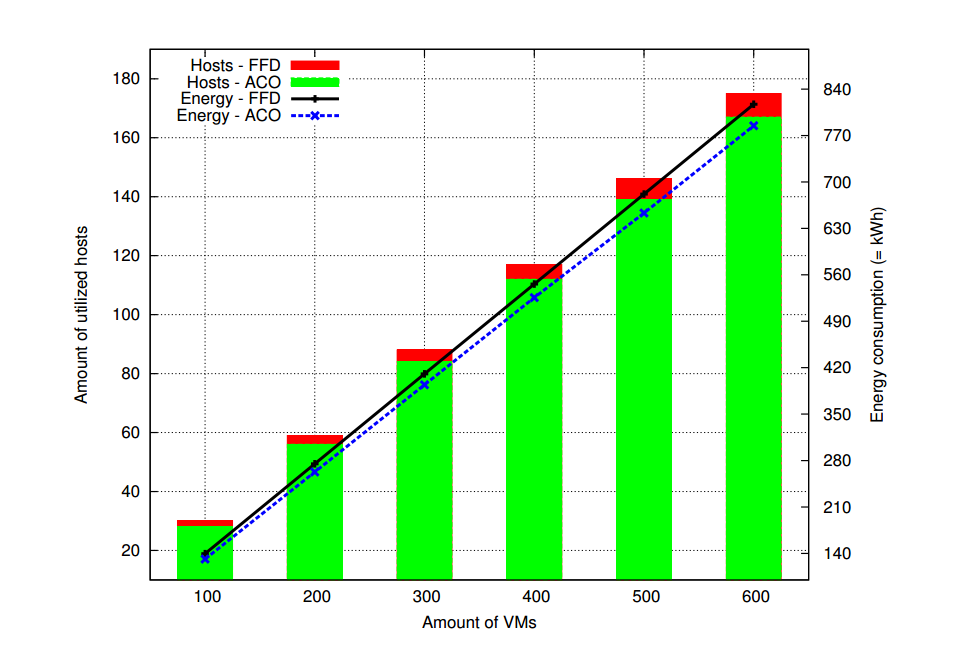
\includegraphics[width=0.8\textwidth]{./Images/antcolonyperf.png}
	\caption{Comparison between First Fit Decreased and Ant Colony algorithms in~\cite{algoAntcolony2}}
\end{center}
\end{figure}

The simulation shows that the ant colony gets better performance than a simple greedy First
Fit Decreasing, however this improvement is not free:

\begin{figure}[H]
\begin{center}
	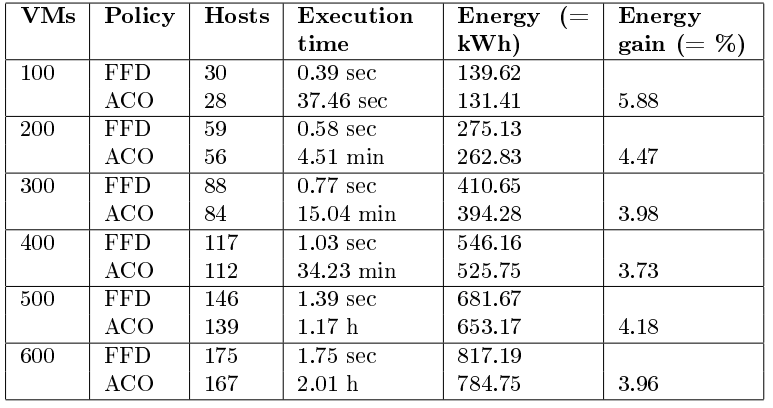
\includegraphics[width=0.6\textwidth]{./Images/antcolonyruntime.png}
	\caption{Runtime of First Fit Decreased and Ant Colony algorithms in~\cite{algoAntcolony2}}
\end{center}
\end{figure}

When the number of nodes becomes bigger, the time spent to find the optimal
allocation grows hugely, it is thousands times longer than a simple First Fit
Decreasing for 3 to 5 percents of improvement. For analysis purpose it is
something interesting to get better results, but in a realistic point of view,
this operation can not take several hours as it should be repeated often.

\subsubsection{Genetic algorithms}

Genetic algorithms (GA) are heuristics based on natural selection. Generations
of solutions are mutating, inheriting with and from each other to result in
close to optimal results.~\cite{algoGenetics1} and~\cite{algoGenetics2}
focused on them to solve the virtual machines assignment problem. In the work
of David Wilcox et al.\cite{algoGenetics1}, simulations are comparing GA with
*-Fit algorithms.

\begin{figure}[b!]
\begin{center}
	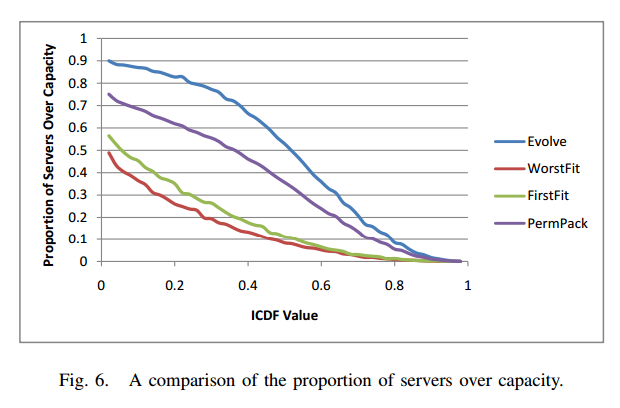
\includegraphics[width=0.65\textwidth]{./Images/geneticperf1.png}
	\caption{Results of simulations using a genetic algorithm\cite{algoGenetics1}}
\end{center}
\end{figure}

\begin{figure}[H]
\begin{center}
	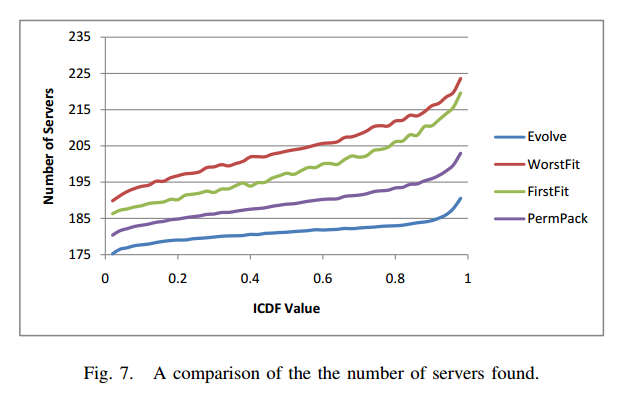
\includegraphics[width=0.65\textwidth]{./Images/geneticperf2.png}
	\caption{Results of simulations using a genetic algorithm\cite{algoGenetics1}}
\end{center}
\end{figure}

On the following graphs, ICDF stands for “inverse cumulative distribution
function” also known as “quantile function”, the authors use it to represent
the load: “Using the icdf, we can specify a percentile value and obtain a
corresponding load which can be passed to the assignment algorithm”.

The conclusion which is that GA tends to consume less physical hosts, at any
load, the number of PMs is largely under the amount of servers used by the
other bin packing algorithms. As a direct consequence, the PMs which are
over-capacitated (where the amount of VMs exceed the resource capacity of the
physical sever), is much more high. For this reason, this approach can hardly
be used in environment where a SLA (Service Level Agreement) has to be
respected, because if there are overloaded servers, some applications or tasks
running of them will be slowed by this situation.

\subsubsection{Network flows}

Network flows are basically directed graphs where each edge has a capacity and a flow.
The main property is that each node of this graph must have an equal sum of flows from
the edges directed to it and leaving from it, except for two particular type of nodes:
“the source node” and “the sink node”.

\begin{figure}[H]
\begin{center}
	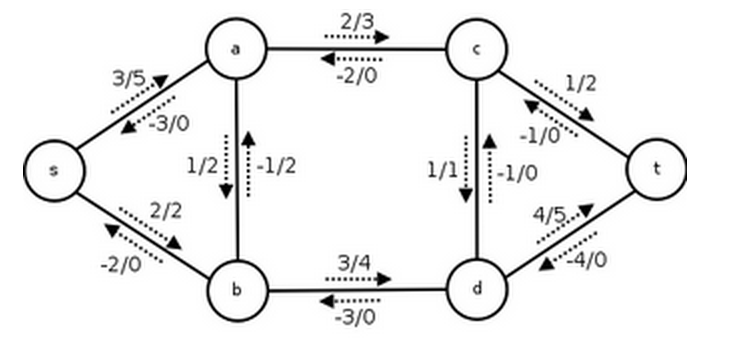
\includegraphics[width=0.8\textwidth]{./Images/examplenetwork.png}
	\caption{Example of network flow directed graph}
\end{center}
\end{figure}

Some people have used this concept to build a model to solve the resource
allocation problem, to fine a close to optimal solution. Kimish Patel, Murali
Annavaram and Massoud Pedram worked on resource assignment in
datacenter\cite{allocationNetworkflow}, considering an heterogeneous
environment as in~\cite{allocationHeterogeneous}. Each set of similar servers,
considered as a pool of servers is represented by a node, with a capacity
different from each other according to the differences between two pools of
servers.

Unfortunately, this technique does not seem to be used for virtual machines
allocation, and the link between this method and the problem we are dealing
with is not obvious at all.

\section{Real data analysis}

Most of the cited works in the literature review are basing their work on
simulations.  In the experiments, simulation tools like
SimGrid\cite{websiteSimgrid} or CloudSim\cite{websiteCloudsim} are used to simulate
the behavior of one or multiple cloud infrastructures.

The data may be generated randomly or following some statistical rules, but
often, workloads are based of extract of real workload. Typically, Google is
releasing workloads of its own production infrastructure. 

In 2012, Google sponsored the ROADEF contest (Operational research and decision
support French society)\cite{websiteRoadef}. The contest was focusing the machine
reassignment problem based on Google workload. Each attendee had to find the
best solution find solution. Some of them resulted in an official publication
like “Heuristics and matheuristics for a real-life machine reassignment
problem” from \citet*{roadefIp}.  They based their work on linear programming.
However in~\cite{roadefBp1, roadefBp2}, the authors have used
around the bin packing algorithms. Unfortunately, the work of the winner has
not been published so we are not able to see which algorithm has been used to
achieve the best reassignment.
 % Introduction
\chapter{Container load balancing in cloud environment}
\label{mainidea}
\lhead{Chapter 2. \emph{Container load balancing in cloud environment}}

\section{Containers - Operating System-level Virtualization}

\subsection{Definition}

The technology of the operating system-level virtualization is composed of
different mecanisms to create isolated environments in the user-space.  Each of
those environment can gather one or several running applications and has access
to different resources. Those environment are commonly called containers from
the tool which popularized them: LXC (LinuX Containers). This technology is 

Operating system-level virtualization has been existing for a long time, it
appeared first in the BSD kernel (1998), where the technology is called
\textbf{Jails}.  Then, Sun developed Solaris (Sun UNIX operating system)
\textbf{zones} in 2005, the same year as the \textbf{OpenVZ} implementation for
the Linux kernel.

Containers are running over the same operating system as the host system, they
are sharing the same drivers, but all the processes contained in them are
limited by this same operating system. The memory consumption, the CPU usage,
the network and disk IO are monitored and managed by these container engines
sending the corresponding instructions to their respective kernel. 

This is a completely different approach to process isolation compare to
classical virtual machines. Where hypervisors and VM have been following the
paradigm where everything is virtualised, creating overhead and slower
performance, then we look at optimising by accessing hardware in order to
reduce binary translations and other slow operations. The main idea for
containers is, based on the host operating system, only the required
devices/features will be virtualised, and finally the level of performance is
close to native efficiency.

\begin{figure}
	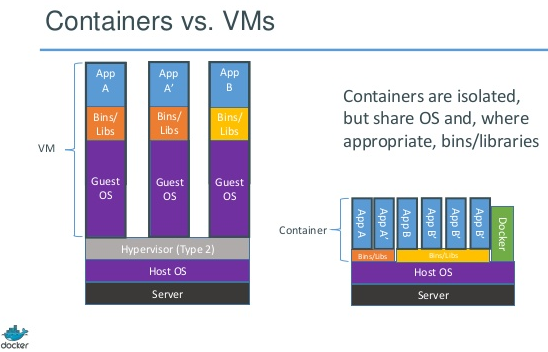
\includegraphics{./Images/containers_vs_vms.png}
	\caption{Structural difference between containers and VMs}
\end{figure}

\subsection{Advantages}

Studying containers is not a random choice, they

\subsection{Limits}

Containers are not able to live-migrate from one host to another with a
standard linux kernel yet. This feature is possible with a OpenVZ patched
kernel because thoses patches implement the checkpoint/restore operations for
the containers, but for a vanilla Linux kernel, it does not exist yet. Some
developers/hackers are trying to clean the code of OpenVZ and push the features
to the mainstream kernel with the \cite{websiteCRIU} project, but so far the
results are mostly drafty and unstable.

This main limit results in the difficulty to host stateful applications like a
database. It can be isolated in a container but we don't have the possibility
to move it without any downtime, the container has to be stop first then
restarted on another host. This is particularly blocking in the case of
production environment where every downtime leads to money loses for instance.

\section{Load balancing and scaling}

As stateful applications can not be cleanly load balanced among a set of
servers, the load balancing of stateless applications will be targeted. More
precisely, web applications.

\subsection{Web Application}

A Web application is an applicative server which uses the web standards to
communicate with clients. There are two main types of web services. The
websites, which are rendering HTML/JS/CSS web pages to users, and web services
defining an API and answering with standard data formats like XML or JSON. Both
of them are using HTTP as transfer protocol.

By the nature of HTTP, web applications are mostly stateless. Each resource
request is done using a new connection (except the case of reusing opened
connections). When a web application is stateful it is linked to the
application itself which is linking information to a local session or
connection.

These last 5 years, more and more of the web services have been written based
on some or all the principles of the REST method which declares as 'best
practice' to create complete stateless applications. Additionaly, another
manifesto, the \cite{website12Factors} has become another standard set of good
practices for web development (website and web services)

The main advantage of stateless services is that they are able to scale
horizontaly easily: the first step is to spawn new instances of the service,
and then modify the routing table of a frontal reverse-proxy. As a result the
requests will be distributed among all the instances.

\subsection{Job balancing on the infrastructure}

When a web application has to be moved from one host to another, there should
be no unavailable time and the current requests have to stopped gracefuly. To
solve the first issue, the following walkthrough has to be followed:

\begin{enumerate}
	\item{Create a new instance of the application - Instanciate a new
	container of a web application}
	\item{Wait until the instance is available - TCP ping the application
	until a connection is established}
	\item{Change reverse proxy routing to route requests to the new
	container and not the old one}
	\item{Stop the old container to free its resources}
\end{enumerate}

To solve the second issue, it should be handle by the application itself. When
the system is querying the old container to stop. It actually sends a signal to
it.  In most systems (Systemd, Upstart at the system level, or Heroku and
Dotcloud at the PaaS level), SIGTERM is sent, then the application has some
time to shutdown. In the case where the application is still running a while
after receiving the signal, SIGKILL is sent to get rid of the process.
 % Background Theory 
\chapter{The experiments}
\label{experiments}
\lhead{Chapter 3. \emph{Experiments}}

\section{Study of the ability to isolate containers CPU usage using Linux control groups}
\subsection{Goal of the experiment}

Linux containers are sharing the same operating system, they are not fully
isolated as we can see with complete virtual machines. To achieve this
isolation, the control groups (cgroup) of the linux kernel are used to
apply limits on the resource access right of each container.

This experiment aims at studying how these cgroups are working and how
do they actually share the CPU resources among the different containers.

\subsection{Metrics}

\subsubsection{Inputs}

The number of CPUs that an application consumes has to be clearly defined. In
each container, an application developped to consume a given number of CPU
cores will be launched. The source code of the application can be found at
\url{https://github.com/Soulou/msc-thesis-cpu-burn}.

\vspace{1em}

\lstset{language=bash}
\begin{lstlisting}
# Parameter n: Number of core to consume
./msc-thesis-cpu-burn -nb-cpus=<n>
\end{lstlisting}

The second input corresponds to the number of shares a container can access
on the CPUs of the running computer. This number is arbitrary as the shares
are relative to each other. 

\begin{quote}
If a container does not have any cpu share number specified, the default value
is: $1024$
\end{quote}

It is expected that if there are two containers, one with $1024$ cpu shares and
the other with $2048$ CPU shares, the second container will have access to
$2048/1024 = 200\%$ of the resources, for a single CPU: $33\%$ and $66\%$.

\subsection{Setup}

\subsubsection{Hosts}

To test the capacity of the isolation by cpu shares, two different environments
will be used. As the result are expected to be relative to the hardware their
should not be any major differences between both, but as a sanity test, it is
important execute it on two différents contexts

The first one my personal laptop, here are its caracteristics:

\begin{itemize}
	\item{CPU: Intel\textregistered \hspace{1pt} Core\texttrademark
	\hspace{1pt} i7-3537U CPU @ 2.00GHz (2 cores with hyperthreading)}
	\item{Memory: 8 GB RAM DDR3}
	\item{Disk: 256GB Solid State Drive}
\end{itemize}

Then we'll study the results of the same experiment on a 4 cores virtual
machine based on an OpenStack cluster:

\begin{itemize}
	\item{CPU: 4 KVM vCPUs}
	\item{Memory: 8 GB RAM}
	\item{Disk: Virtual HDD 80GB}
\end{itemize}

\subsubsection{Deployment}

In order to simplify the reproduction of these experiments, the different
applications have been packaged into container images. They can be found on the
docker public repository:

\begin{itemize}
	\item{\texttt{soulou/msc-thesis-cpu-burn}}
	\item{\texttt{soulou/msc-thesis-docker-cpu-monitor}}
\end{itemize}

In order to deploy them, simply install Docker on your host
(\url{http://docs.docker.com/installation/}), then use the \texttt{docker pull}
to get the container images locally.

\vspace{1em}

\begin{lstlisting}
docker run -d soulou/msc-thesis-cpu-burn -nb-cpus=<n>
...
# Run more instances according to what your want to test
...
docker run -i -t \
  -v /var/run/docker.sock:/var/run/docker.sock \
  -v /sys/fs/cgroup/cpuacct/docker:/cgroup \
  soulou/msc-thesis-docker-cpu-monitor -cgroup-path=/cgroup
\end{lstlisting}

The cpu monitoring service will display in columns the cpu consumption
of each container running on the host (including itself), the data are
displayed to be quickly usable by a third-party data analysis tool like
\textbf{R} or to draw graph with \textbf{Gnuplot}

\subsection{Expected results}

Four different experiments have been done:

\begin{itemize}
\item{4 Processes with equal CPU shares : \newline The tested hosts
	have a total of 4 cores, normally 4 processes using 1 core each should
	be able to share it equaly, and each of the process should be able to
	get 100\%
}
\item{4 Processes with different CPU shares 128-256-512-1024 : \newline
	For the same reason as the previous experiment, the
	shares should not change the results. Even if some processes have less
	priority over the CPU, as there is enough cores for all the processes,
	they should all be able to run their process at its maximum potential.
}
\item{6 processes with equal CPU shares : \newline This case is
	different, as there is a higher number of processes compared to the
	amount of available computation units. With an equal amount of CPU
	shares for each process, it is expected that each process will get 66\%
	in average of CPU time.  The results can't be stable as the mount of
	cores is not a divisor of the number of applications. In other words,
	there is no way the operating system can allocate an equal share of
	core per process, as the context of a process is linked to one core. An
	application can't be 33\% on one core, and 33\% on the other one at the
	same time.
}
\item{6 processes with different CPU shares 32-64-128-256-512-1024 : \newline
	According to the rule defined previously, a process with 64 shares
	should have twice more CPU time than a process with 32 shares but twice
	less than a 128-shares process.
}
\end{itemize}

\subsection{Results}

All the following graphs represent the percentage of CPU time per process
in function of the time in seconds.

\subsection{On the laptop}

\begin{figure}[h!]
\begin{center}
	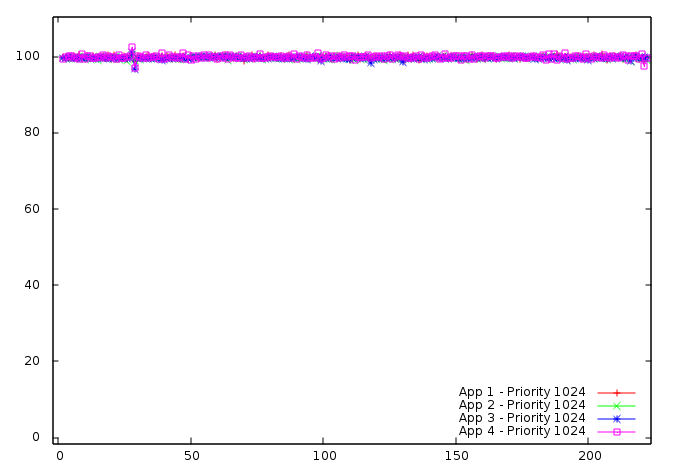
\includegraphics[width=0.45\textwidth]{./Images/CpuMonitor/laptop/4_equalshares.png}
	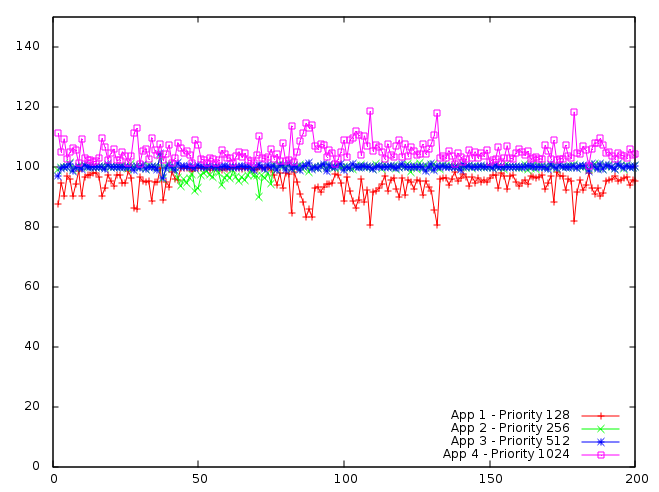
\includegraphics[width=0.45\textwidth]{./Images/CpuMonitor/laptop/4_differentshares.png}
	\caption{4 Processes with equal[1] and different[2] CPU shares}
\end{center}
\end{figure}

Using 4 processes, the expectations are reached, even if there are some small
differences between the excution with equal shares and the one without, it is
clear that each service can use one complete core whatever are its CPU shares.

\begin{figure}[h!]
\begin{center}
	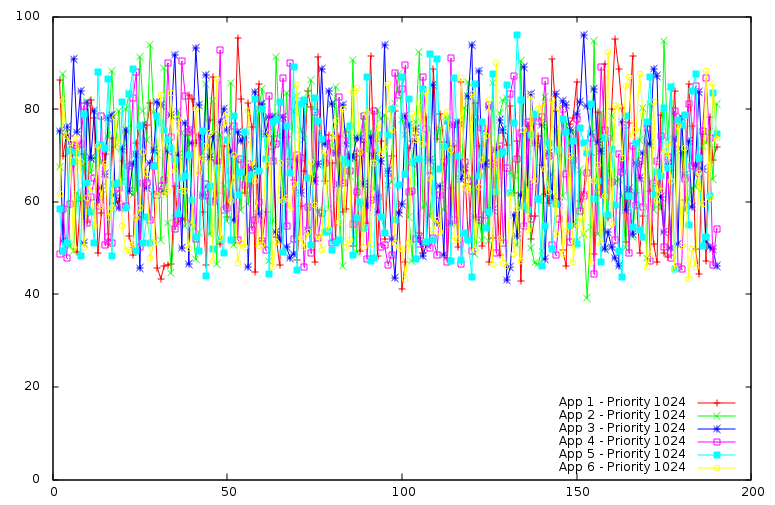
\includegraphics[width=0.45\textwidth]{./Images/CpuMonitor/laptop/6_equalshares.png}
	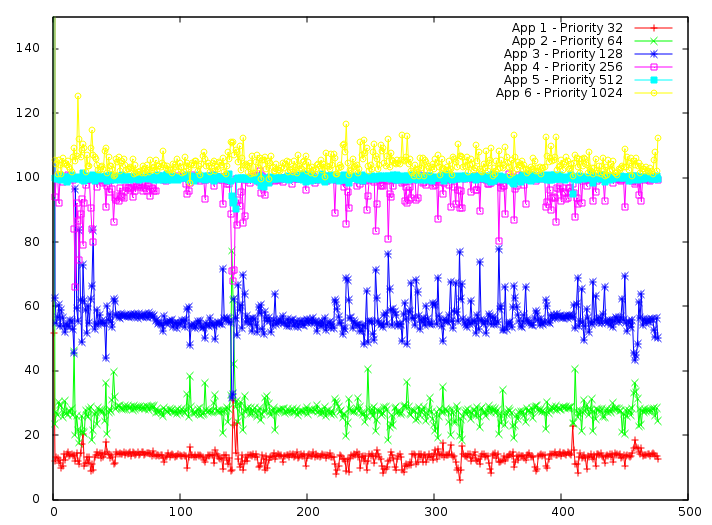
\includegraphics[width=0.45\textwidth]{./Images/CpuMonitor/laptop/6_differentshares.png}
	\caption{6 Processes with equal[1] and different[2] CPU shares}
\end{center}
\end{figure}

When 6 processes are executing on the host the observed behavior is different.
When shares are equal, the cpu consumption of each process is completely
unstable.  As explain in the expectation for this experiment, theoretically
each process should have 66\%, but as it's not possible because a process is
only attached to one core at a precise time, the operating system is moving the
processes during all the calculations. This is why the curves are so changing.
But overall, if we measure the average and median of the CPU consumption of
each application, the result is 66\%, so the expectation is reached.

In the case where 6 processes are running with different CPU shares, the
results are linked to what has been planned, but not only. The process with the
minimum amount of shares (32) is using $\approx15\%$ of CPU, then the one with
64 shares has $\approx30\%$ of CPU consumption, and then, the third one has
$\approx60\%$ of processor usage. These values are effectively each time twice
higher as the previous one. However this rule is not respected afterwards. Three
of the process are able to use one full core event if their shares are respectively
really different (256, 512, 1024)

\subsection{On the virtual machine}

As previously said, the results of this experiment in another environment should
not be fondamentally different. As the results are relative percentages, the
same figures should be found.

\begin{figure}[h!]
\begin{center}
	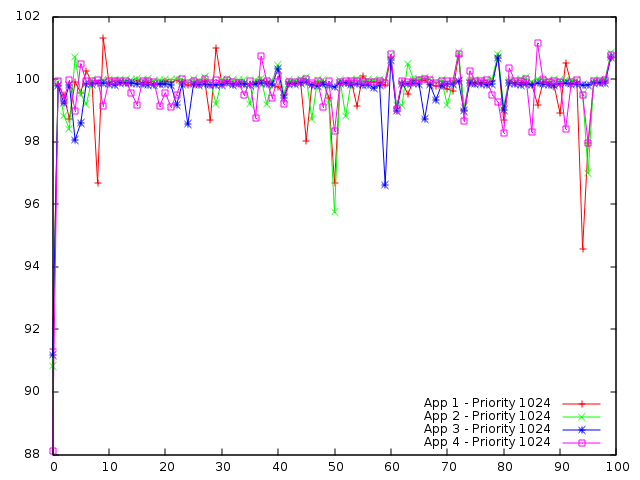
\includegraphics[width=0.45\textwidth]{./Images/CpuMonitor/vm/4_equalshares.png}
	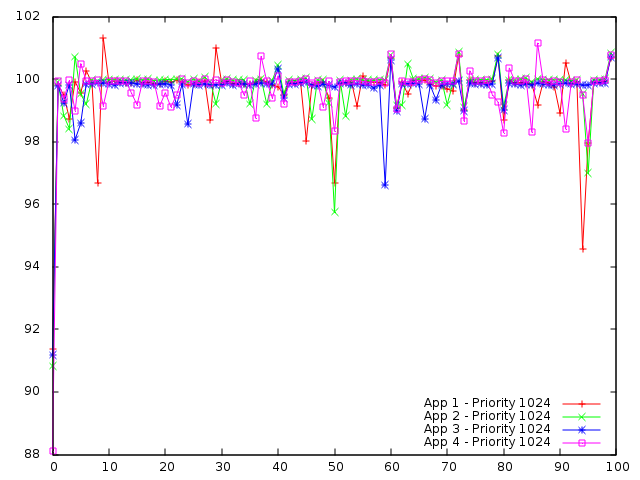
\includegraphics[width=0.45\textwidth]{./Images/CpuMonitor/vm/4_differentshares.png}
	\caption{4 Processes with equal[1] and different[2] CPU shares}
\end{center}
\end{figure}

For 

\begin{figure}[h!]
\begin{center}
	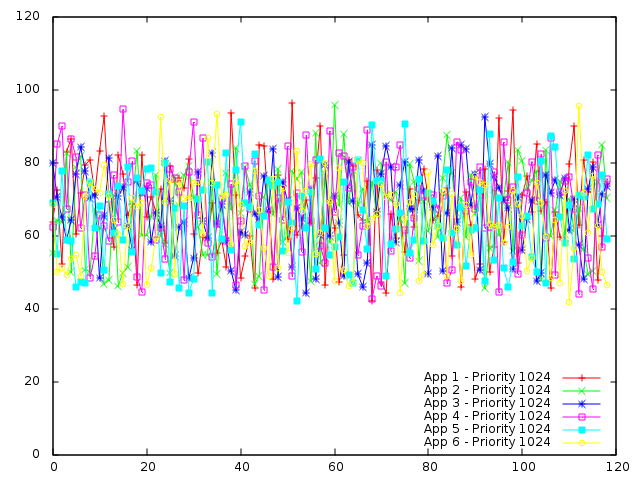
\includegraphics[width=0.45\textwidth]{./Images/CpuMonitor/vm/6_equalshares.png}
	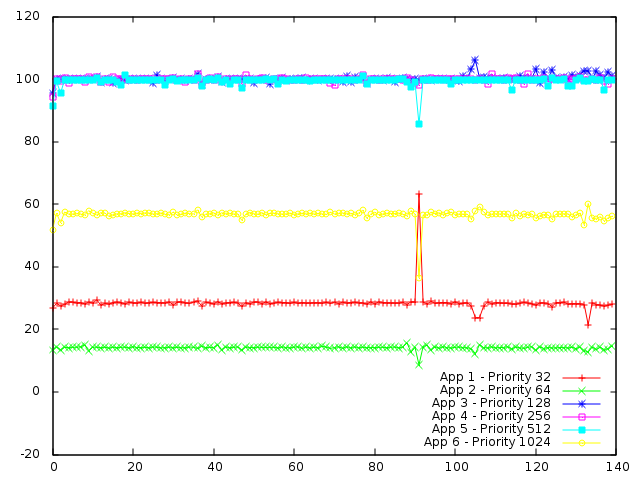
\includegraphics[width=0.45\textwidth]{./Images/CpuMonitor/vm/6_differentshares.png}
	\caption{6 Processes with equal[1] and different[2] CPU shares}
\end{center}
\end{figure}

Ipsum lorem dolor sit amet

\subsubsection{Comments on the results}

\subsection{Conclusion on the experiment}
 % First experiment: CPU isolation
\chapter{Definition of the experimental setup}
\label{chap:expsetup}

This chapter will be devoted to the study of the containerized web application
allocation and load balancing in a cloud environment. Before speaking of the
experiments themselves, it is important to define how those experiments have
been setup. The target is the ability to test algorithms using a realistic
infrastructure and not to create a simulation of it.

\section{Hardware Infrastructure}

Different kind of clouds are coexisting, if \textbf{Amazon Web Services} provides
services which are part of a “public” cloud, this is not the only way to use a
cloud infrastructure: private cloud or hybrid clouds mixing private and public
cloud infrastructures are being developed more and more. Thanks to open-source
projects like~\cite{websiteOpenstack}, cloud environments can be installed on
private infrastructures.

The experiments have been done on a private cloud infrastructure, powered by
Openstack (version: Grizzly). But they could be equaly executed on a public
cloud, or event bar metal servers. The amount and the capacities of the virtual
machines have been different according to the experiment, but all the instances
are always in the same private network.

This document won't cover how to install Openstack but there are plenty of
tutorials on the web. Moreover this setup can be done in a public cloud
infrastructure like Amazon Web Services EC2, there is no difference. We are
going to use two distinct kinds of node. The agents execute the
different web applications, and the controller which is the interface to
control the complete infrastructure.

\section{Software Infrastructure}
\subsection{Operating System}

All the virtual machines are running \textbf{Ubuntu Server 14.04 LTS}, this choice
has been lead by the fact that this Linux distribution is probably the most standard
worldwide and because \textit{python 3.4} is required to run some libraries of the project
to execute the experiments.

The cloud version of the distribution has been chosen\footnote{Download page of
Ubuntu 14.04 Cloud :\url{http://cloud-images.ubuntu.com/releases/14.04/}} if
order to be compatible with Openstack and correctly boot. To add the image to
an openstack cluster, only one command is required:

\vspace{1em}
\begin{lstlisting}
glance add name="ubuntu-trusty" is_public=true \ 
  container_format=ovf disk_format=qcow2 < /path/to/file.img
\end{lstlisting}

To deploy, run, stop and migrate our applications, \textbf{Docker} will be
used. More precisely its REST API. Actually all the requests to Docker are done
through HTTP requests on a unix socket. (\textbf{Docker} is using a unix socket
owned by root for security reasons, to avoid remote access to the host)

\subsection{Service discovery}

One of the common difficulties in cloud infrastructure gathering numerous
virtual machines is the service discovery. It is possible of course to use a
configuration manager to generate static configuration on each node which will
be used by the different services. However this system is static, doesn't scale
well and is not fault resilient. That is what it is a bad idea to write
anything statically when deploying such infrastructure.

The project \textbf{Consul} has been used to achieve the feature. Consul is
decentralized solution for service discovery based on two protocols. On the one
hand, it is using a gossip protocol to manage the communication between nodes.
This feature let \textbf{Consul} creates a decentralized cluster of servers.
When a new node is available, it just needs to communicate with one node,
whichever it is, to join the complete cluster and get access to the shared
resources. On the second hand, the process is using a consensus algorithm to
elect a leader node on the cluster, which has the responsibility to keep the
data consistent. Write operations have to be validated by the leader node, then
spread to the rest of the servers. If the leader node crashes, another node is
automatically elected by the others nodes.

\textbf{Consul} main usage is service discovery, so each node is registering its
running services to consul which will spread the information among the whole
cluster. That is how services get to know each other.

The application is developed using the \textbf{Go} programming language, so
the installation is trivial. To achieve the installation, whatever is the
operating system, downloading the binary from the website
\url{http://www.consul.io/downloads.html} and executing it enough.  The
configuration of each node service is done through a set of JSON files which
have to be defined in \textbf{Consul} configuration directory.

\subsection{Balancer agent}

On each server which has to execute the web applications, the installation
of the balancer agent is required. It is a HTTP server written using python3.
The source code can be found on GitHub
\footnote{\url{https://github.com/Soulou/msc-thesis-container-balancer-agent}}. The
installation is straightforward.

\vspace{1em}
\begin{lstlisting}
git clone \
  https://github.com/Soulou/msc-thesis-container-balancer-agent
cd msc-thesis-container-balancer-agent
virtualenv -p /usr/bin/python3 .
source bin/activate
pip install -r requirements.txt
\end{lstlisting}

As the agent has to communicate with \textbf{Docker} is should be run as
root:

\vspace{1em}
\begin{lstlisting}
sudo -E python agent.py
\end{lstlisting}

The server has two distinct roles. The first one is to execute instructions
coming from a controller, the interface is an HTTP API. You can find its
documentation in the Appendix A: ~\nameref{app:agent-api}

The other role of the agent is to achieve real time monitoring of the
server itself and of each container running on it. Different threads
starts in parallel with the HTTP Server. The reason why it is necessary
to use separate threads is that at a given time it's not possible to
get some relative data. This is how the different metrics are gathered
by the agent.

For the entire server:

\begin{itemize}
\item{CPU: The interface from the Linux Kernel to read the CPU usage is
\texttt{/proc/stat}. When this virtual file is read, the kernel fills it with
the current information about the CPU usage, the interruptions and the
processes. However those data are cumulative. So each second the data are
fetched, and compared to the CPU usage of the previous second. The data are un
\textit{User Hz}, this unit represent a tick in the user space, 100 of them are
generated per second, so the value shown in this file are close to hundredths of
second.} \item{Memory: This value is easier to access, the kernel provides
\texttt{/proc/meminfo} which contains the real time data usage. There is no
extra work to do in order to the clean pieces of information.} \item{Network
I/O: \texttt{/proc/net/dev} contains all the information related to all the
network interfaces of the server, in this file is displayed the amount of bytes
and packets sent and received by each of them. The values are also cumulative,
that's why the agent has to keep track of them. As a result when a request is
done to get the system usage, the right data can be sent directly and it's not
required to wait 1 second.}
\end{itemize}

For the containers:

\begin{itemize}
\item{CPU: The CPU usage of each container is accounted separately thanks to
the \textit{cpuacct} cgroup feature of the Linux Kernel. The communication
from the userspace is done through a virtual file system located at
\texttt{/sys/fs/cgroup}. As a result, for docker we can find the correct data
at that path: \newline\texttt{/sys/fs/cgroup/cpuacct/docker/:container\_id/cpu.usage}.
As precedently, the value is in \textit{User Hz}, so the process to calculate the
actual CPU usage is similar as the \texttt{/proc/stat} analysis.
\item{Memory: The cgroup \textit{memory} manages the memory usage and limits per
container, it is enough to read
\textit{/sys/fs/cgroup/memory/docker/:container\_id/memory.usage\_in\_bytes} to get
the interesting piece of information.}}
\item{Network I/O: It is a bit more difficult to monitor the network usage of a container,
as the resource management mechanisms is not part of the cgroup, it is another feature
of the Linux Kernel called "network namespace". In order to get access to it, different
steps are required.
\begin{enumerate}
\item{Find the PID of a process in the monitored container by looking in \texttt{/sys/fs/cgroup/:cgroup/docker/:container\_id/tasks}}
\item{Access the network namespace file located in \texttt{/proc/:pid/net/ns}}
\item{Create a link of this namespace to \texttt{/var/run/netns/:container\_id}}
\item{Use IP command to get stats from the desired namespace \texttt{ip netns exec :container\_id netstat -i}}
\end{enumerate}}
\end{itemize}

To sum up, three distinct threads are running in the Balancer agent, the HTTP
server, the host system monitoring, and the containers monitoring. Those
threads are used to be able to get accurate data instantly, otherwise 1 second
should be waited to get interesting data.

\footnote{\url{https://github.com/Soulou/msc-thesis-container-balancer-agent}}

\subsection{Balancer controller}

The second main brick of this infrastructure is the controller. The role of
this software is to control all the different agents, to give them the
instructions about which container to start and which container to stop. There
is no need to configure this service particularly, the knowledge about the
composition of the infrastructure is acquired through requests to the local
\textbf{Consul} agent.

The running applications on the cluster are gathered by \textit{service}. Each
of them can contain a variable amount of containers hosted on the different agent.

Moreover, it updates dynamically the routing tables of the different services
running on the infrastructure. If a service called "service-test" owns two containers,
the incoming requests will be routed to both of those containers by following a
round-robin algorithm. (C1 - C2 - C1 - C2 - ...).

\textbf{Hipache}\footnote{\url{https://github.com/dotcloud/hipache}} is used as
a front HTTP working as reverse proxy, it is in charge of routing incoming
requests to the different containers.  Why \textbf{Hipache} has been used
instead of a more classical server like \textbf{Apache}. The main reason is
that \textbf{Hipache} is dynamically configurable thanks to different backends.
The most common is the \textbf{redis} backend. \textbf{Redis} is a key-value
store with really high performance as all the dataset stay in memory, and is
asynchronously written to the disk. So when the controller sends request to
start or stop a container, it also connects to a \textbf{redis} instance to
update hipache configuration.

The controller also exposes a HTTP API which is described in the Appendix
B~\nameref{app:controller-api} Part of this API is only a proxy to the agents
endpoint, in order to gather all the data to only one location, and  on the
other side, there are the active actions, linked to container scheduling on the
infrastructure.

This component of the infrastructure is critical for the experiment detailed
later in this work. The controller is charged to choose the nodes where the
containers have to start. To select a strategy which will be used when a new
controller has to start, it has to be specified as options:

\begin{lstlisting}
python3 controller.py --strategy random
\end{lstlisting}

In the previous example, the new containers will be placed randomly on the different
available nodes. Others strategy are available:

\begin{itemize}
\item{random: Choose randomly a node}
\item{round-robin: Choose one node after the other, following a loop:
\begin{figure}[h!]
\begin{center}
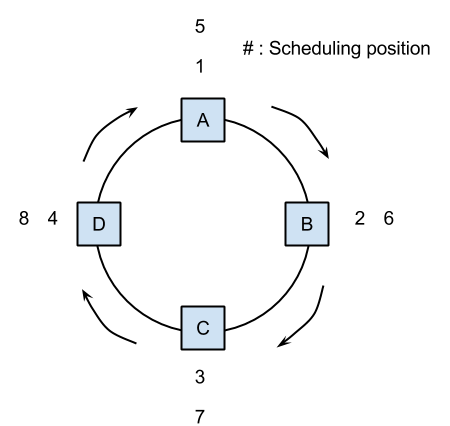
\includegraphics[width=0.5\textwidth]{./Images/round-robin.png}
\caption{Scheme of a round-robin scheduling}
\end{center}
\end{figure}}
\end{itemize}
 
\footnote{\url{https://github.com/Soulou/msc-thesis-container-balancer-controller}}

\subsection{Balancer client}

The balancer client, is a command line tool to command the controller, it
shows in a human-understandable way, the JSON results the controller and allows
a user to execute requests easily. Its documentation can be found in the
Appendix C: "~\nameref{app:client-doc}".

\footnote{\url{https://github.com/Soulou/msc-thesis-container-balancer-client}}

\subsection{Deployment}

All those services and tools have to be deployed on the instances of the
infrastructure.  More and more configuration managers (CM) are released those days to
answer the increasing needs to deploy applications in volatiles infrastructure,
composed of temporary virtual machines. To setup all the different pieces of
this infrastructure, \textbf{Ansible} has been used. There are two main models
of CMs, those centralized around a server, like \textbf{Chef Server} or \textbf{Puppet},
where the nodes synchronize themselves with this server. The devops do not connect
directly to the nodes but give instructions to the central server. The second
category are those who are run from a devops workstation, like \textbf{Chef Solo},
\textbf{Ansible}, \textbf{SaltStack}. The choice of \textbf{Ansible} has been done
for it's ability to deploy nodes in parallel and by it's easiness of prototyping,
its syntax is pretty simple.

All the mecanisms of deployment can be found on following \textit{GitHub} page:
\url{https://github.com/Soulou/msc-thesis-cloud-builder}. The script requires
that \textbf{Openstack} credentials are stored in environment variables. (
\texttt{OS\_USERNAME, OS\_TENANT\_NAME, OS\_PASSWORD, OS\_AUTH\_URL,
OS\_REGION\_NAME}). Then it uses the API to instantiates VMs, and then deploy
all the services on them using ansible \footnote{Ansible configuration:
\url{https://github.com/Soulou/msc-thesis-cloud-builder/tree/master/ansible}}.

 % Design of the platform
\chapter{Study of algorithms for containers allocation and load balancing}
\lhead{Chapter 5. \emph{Study of algorithms for containers allocation and load balancing}}
\label{chapt:containerloadbalance}

\section{Experimental applications}

The experimental process aims at measuring the performance of a set of
containers before and/or after using any resource allocation algorithm. First,
we have to define which applications will be containerized for those
operations. Those applications have to be deployed on all the agent servers and
have to behave as standard web services. Whatever is the language or the
framework used (except PHP), all the dependencies of the applications are
loaded on application startup, so afterwards, there is no more file to read
from the disk. It results in low input/output for most of the applications and
this metric will not be measured.

The first service which has been used during the experiments is an application which
is calculating $N$ elements of the Fibonacci suite\footnote{\textbf{Docker}
image: \texttt{soulou/msc-thesis-fibo-http-service}}. This web application has
only one endpoint: \texttt{GET /:n}, which returns the $N^{th}$ items, of the
Fibonacci sequence. This application only consumes CPU, the memory footprint is
really negligible.

The second application has been designed to consume a precise amount of
resource during a specified duration\footnote{\textbf{Docker} image:
\texttt{soulou/msc-thesis/memory-http-service}}. Its endpoint is \texttt{GET
/:memory/:time} with the memory in megabytes and the time in milliseconds. For
instance, \texttt{GET /10/100} will consume precisely 10MB for a duration of
0.1s. Thanks to this application, we can measure precisely how much should
consume the application with a load of $N$ requests per second of a certain
amount of memory during a precise timelapse.  The memory is allocated and
initialized. As a result, even if we are requesting amount of memory, it also
generates an important CPU load in the loops for memory application.

The source code of both services can be found on \textbf{GitHub}:
\begin{itemize}
\item{\url{https://github.com/Soulou/msc-thesis-fibo-http-service}}
\item{\url{https://github.com/Soulou/msc-thesis-memory-http-service}}
\end{itemize}

\section{Load generation}

An important question when measuring performance is the way to generate the
requests. Do they have to reflect a realistic user load, is it possible to do
it, is it pertinent? In this case, we are going to measure raw performance
over the cluster, to gather data about the efficiency of a specific algorithm.
When user load simulation algorithm is used, the benchmark is irregular, and
finally getting information about the real impact of a given algorithm may be
more difficult to do.

\subsection{Tools}

To generate web traffic, HTTP requests generators are required. Historically,
the most used tool is part of the \textbf{Apache} web server tools, and is
called Apache Bench \textit{Command line name: ab}, released under the
open-source \textit{Apache Licence}. This utility is not really used anymore
because it is single-threaded which. This is a very limiting caracteristic,
only one CPU core is used, it may not be enough to saturate a target and get a
correct measure of the performance.

The tool which has been mostly used in the scope of this work is named
\textbf{wrk}\footnote{\url{https://github.com/wg/wrk}}. This is a benchmark
tool able to send requests using a given number of connections, used in
different parallel threads. (The opposite of \texttt{ab}, which sends all
the request concurrently using one thread)

Usage example:

\vspace{1em}
\begin{lstlisting}
wrk -c 10 -t 2 -d 1m http://service1.thesis.dev
\end{lstlisting}

This example will send 10 requests concurrently during 1 minute using two threads.
So we are sure that the targeted URL will receive a maximum of 10 request at a
given time.

One reproach which can be made to this tool is that it doesn't adjust the
number of threads automatically. By default, two threads are used, but if we
need more parallel connections, the user has to define it by hand. But is most
of the case, giving a thread per core on the underlying computer is the
best practice.

\subsection{Different kinds of load}

Combining \textbf{wrk} and the two previously defined web application, different
kinds of load can be generated. Thanks to the "memory" HTTP service, it is even
possible to emulate different kinds of application.

\subsection{Lightweight services}

In some cases, web applications are micro-services and their job is to do a small
particular task. Commonly, requests are really quick and the treatment of each of
them has a low memory footprint. However as those HTTP requests may be numerous,
the overall processor and memory usage can be important.

In out infrastructure, one container of such a service may be represented by instances
of the memory services with requests using a few megabytes of memory, are done
really quickly: \texttt{http://micro-service.thesis.dev/5/100}. All the requests to this
endpoint are compliant with the previous constraints. The following data show how 
such application behave in an environment where they don't have to share resources\footnote{All the measure
have been done 5 times, and the given result is  the average}:

\begin{itemize}
	\item{One instance: \newline
	\texttt{wrk -c 20 `http://memory-service.thesis.dev/5/100'} --- 82.05req/s --- CPU 106\%, 24MB \newline
	\texttt{wrk -c 40 `http://memory-service.thesis.dev/5/100'} --- 93.74req/s --- CPU 112\%, 22MB \newline
	There is no big difference when running 20 or 40 connections in parallel, so we can assume that we have
	reached the maximum capacity of the instance. As announced previously, the memory usage is really low, but
	the application is using one complete core.\vspace{1em}}
	\item{Two instances on two different hosts: \newline
	\texttt{wrk -c 20 `http://memory-service.thesis.dev/5/100'} --- 123.23req/s --- CPU 109\% | 80\%, 15MB | 14MB \newline
	\texttt{wrk -c 40 `http://memory-service.thesis.dev/5/100'} --- 165.77req/s --- CPU 117\% | 97\%, 17MB | 31MB \newline
	The exepectations were that two instances would be able to execute twice the number of requests compared to
	the previous case. With 20 connections, it is not the case, but with 40, the service has been able to execute
	165 requests per second, which is more or less the double as previously. 20 connections was not enough. This
	lack can be seen by the fact that the CPU usage of one of the instances is not one complete core but 80\%.}
	\item{Two instances on the same host: \newline
	\texttt{wrk -c 20 `http://memory-service.thesis.dev/5/100'} --- 101.11req/s --- CPU 97\% | 98\%, 17MB | 18MB \newline
	\texttt{wrk -c 40 `http://memory-service.thesis.dev/5/100'} --- 127.77req/s --- CPU 115\% | 117\%, 18MB | 17MB \newline
	The instances have 2 vCPUs, so theoretically two instances of a same service on one node should be able to run
	at maximumal performance, but in practice, the results are not as good, a ratio of 1.5 has been reached using
	40 parallel connections. This is a perfect illustration of a ``bad neighbour'' situation, the performance of
	each container is jeopardized by the other instance. That is something which can be (at least partially) solved
	with scheduling algorithms, to avoid as much as possible this case.}
\end{itemize}

Note: The values of CPU usage are often above 100\% when an application is
using on core.  The amount of \textit{User HZ} is read every second, so it may
be an inacurracy of this timer, or it may be that the time used by the kernel
to schedule processes is taken into account. As a result, the process uses
100\% and the kernel uses some CPU time on another core.

\subsection{Bigger services}

The opposite of previous microservices are more important web services, consuming
more memory per request, with a lower number of request per second:

\begin{itemize}
	\item{One instance: \newline
	\texttt{wrk -c 20 `http://memory-service.thesis.dev/50/500'} --- 10.79req/s --- CPU 122\%, 326MB \newline
	\texttt{wrk -c 40 `http://memory-service.thesis.dev/50/500'} --- 9.30req/s --- CPU 116\%, 293MB \newline
	\vspace{1em}}
	\item{Two instances: \newline
	\texttt{wrk -c 20 `http://memory-service.thesis.dev/50/500'} --- 19.48req/s --- CPU 122\% | 80\%, 259MB | 182MB \newline
	\texttt{wrk -c 40 `http://memory-service.thesis.dev/50/500'} --- 23.26req/s --- CPU 102\% | 98\%, 302MB | 283MB \newline
	\vspace{1em}}
	\item{Two instances on one node: \newline
	\texttt{wrk -c 20 `http://memory-service.thesis.dev/50/500'} --- 19.48req/s --- CPU 109\% | 106\%, 153MB | 170MB \newline
	\texttt{wrk -c 40 `http://memory-service.thesis.dev/50/500'} --- 19.43req/s --- CPU 105\% | 101\%, 202MB | 195MB \newline
	\vspace{1em}}
\end{itemize}

Except the fact he the servers suppor less requests as each of them is heavier,
the behaviour between a light application and this one is prett similar. It
scales out correctly, doubling the mount of requests the service can manage.
With this application even if the memory consumption is getting higher, the
limiting resource is still the processor. The fact that the CPU is in most of
the case the resource causing a bottleneck is something
common.~\cite{reassignmentElectricitysaving, reassignmentVisbp}

In the previous examples we have done performance benchmark, the maximum
performance of the services have been measured. But with \textbf{wrk}, it
is possible to send a lower amount of requests to simulate a normal load.
When 1 to 10 connections are used (instead of 20 or 40) like in the previous
experiment, the resulting CPU consumption would vary respectively 
between 10 and 100\%

\section{Bin packing algorithms}

Bin packing algorithms have been defined in the~\cref{litreview}, but here is a
short reminder about the main ideas behind them.  A bin packing algorithms
consist in packing items into bins. Each bin has a capacity and each item
weighs certain size. There are two main categories: online bin packing and
offline bin packing. The first type is defined by the following setup. The bins
are already filled with items, but we can't have details about those items.
There is a new item to pack, the online bin packing algorithms have to choose
the best bin for the new item.  The offline bin packing algorithms consider
that all the bins are empty, and it has to pack all the items into the bins.
All the information about each item is available.

We speak of bin packing algorithms with the plural, because there isn't only
one way to pack items, offline bin packing is an NP-Hard problem, finding the
optimal solution can be very long. That's why a large number of heuristics
exist to get a good enough result in a short enough period.

\subsection{Relation with resource allocation}

In our situations, the items are the appications containers and the bins are
the different hosts, here OpenStack virtual machines. Different operations
can be done when packing application containers:

\begin{itemize}
	\item{Consolidation: Use the minimum of hosts to run correctly all the containers}
	\item{Load balancing: Balance the load over the available hosts}
	\item{Container Allocation: Choice of the best node to run a new container}
\end{itemize}

First, it is important to define the fact that the resource consumption of a
container is completely ephemeral. As the resources are not completely
dedicated to a container, but shared with each other, the container may have
to be moved soon after its allocation, when its load has been defined. That's
why using only resource allocation is not enough to balance correctly the
infrastructure.

As the consumption of CPU is variable, it is important to keep a security
reserve. If the amount of requests to a container increases, it has to be
able to get more CPU time, otherwise it will the stucked and all the requests
would be impacted. That's why, there is a default margin of 20\% in the
platform we are using. It means that if a server is loaded up to 50\% and
that a new container estimated at 40\% has to be packed. The server wouldn't
be considered as available as the total is over 80\% (for a one core server)

\subsection{Container allocation --- online bin packing algorithms}

\subsubsection{Type of new items}

Online bin packing means that we have to pack new items into bins without
having the knowledge of what is already present in the bins. So bins have a
remaining capacity, and each new items is known or partially known. In some
cases, the new items are completely unknown.

In this infrastructure there are two different cases which can be distinguished:

\begin{itemize}
\item{The new container is part of a new service: there is no information about
the number of incoming requests, and what is the memory footprint of the new process}
\item{The new container is from an existing service: in this case, the CPU consumption
and memory usage can be estimated by looking the other containers of a similar service.
For instance, if two containers of \texttt{service1} are running using both 20\% of CPU,
it is probably true that the consumption of the new container will be capped at 20\%}
\end{itemize}

\subsubsection{Algorithms and Heuristics}

In the following part, different algorithms are going to be used. Some dummy
methods will be used as comparative methods. They are `random' and
`round-robin'. With those strategies, no bin packing is executed, the choice
of the server is determined randomly or through a round-robin loop.

Three basic algorithms of bin packing are used:

\begin{itemize}
	\item{First Fit: The item is packed on the first bin which is able to contain it}
	\item{Best Fit: The bin which is able to contain the item with the smallest capacity}
	\item{Worst Fit: The bin which is able to container the item with the biggest capacity}
\end{itemize}

Our nodes and containers are monitored over three metrics: ``CPU usage'',
``Memory usage'', ``Network I/O''.  As it has been shown previously, the only
resource wich is a bottleneck from far the the CPU\@. As a result the
algorithms have been implemented the following manner: when the item is
inspected to see if it can fit on one node, all the metrics are compared, if
one of them is insufficient, the allocation on this node is rejected. However
in best fit and worst fit, when we need to select the best, or the worst, only
the CPU is considered.

\subsubsection{Experiment - Comparaison of algorithms}

This experiment consists in starting a set of containers using different
algorithms to choose the destination node. There are 8 virtual machines with 2
cores, 7 of them are agents running the container and one is controller and
load balancer to route the HTTP requests to the instances. The containers are
splitted into 3 services of various sizes:

\vspace{1em}
\begin{tabular}{l | c | c | c | c}
	& Number of containers & Memory Usage & Request Duration & Parallel connections \\
	Service 1 & 4 & 10MB & 10ms & 30 \\
	Service 2 & 4 & 25MB & 200ms & 20 \\
	Service 3 & 2 & 50MB & 300ms & 10 \\
\end{tabular}
\label{tab:exp2-services}
\captionof{table}{Description of the experimental HTTP services}
\vspace{1em}

A container has been launched every 5 seconds to let the time to the monitoring
system to take it into account and to be able to measure its usage. The HTTP
requests are sent even before the first container has been created, be cause the
front-end server \textbf{Hipache} will drop the request answering the HTTP error
\textit{502 bad gateway}. As soon as a container from the given service is available
the requests are correctly routed to it.

The metric which is measured is the one important from an user perspective. The
number of requests answered per second. We are expecting worst-fit, random and
round-robin to get better results that first-fit and best-fit because they
don't try to optimize the number of used servers, but they will spread the services
on all of them.

For each algorithm, 5 executions have been done and the displayed value is the average
of the the result of each of the tries. One execution lasts 2 minutes, and the obtained
value is the amount of requests answered per second.

\begin{figure}[h!]
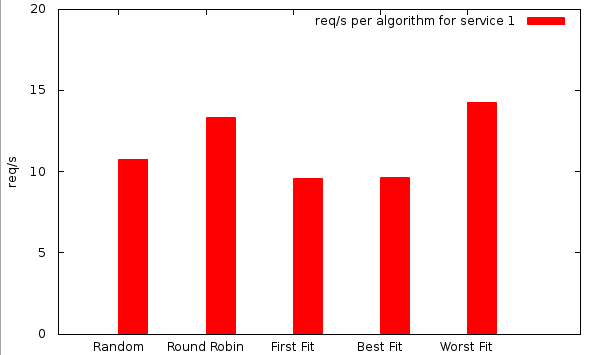
\includegraphics[width=\textwidth]{./Images/BinPacking/exp2-service1.png}
\label{fig:exp2service1}
\caption{Service 1: Number of requests per second for various algorithms}
\end{figure}

\begin{figure}[h!]
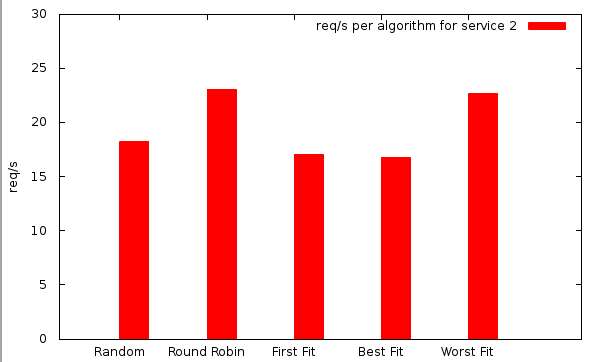
\includegraphics[width=\textwidth]{./Images/BinPacking/exp2-service2.png}
\label{fig:exp2service2}
\caption{Service 2: Number of requests per second for various algorithms}
\end{figure}

\begin{figure}[h!]
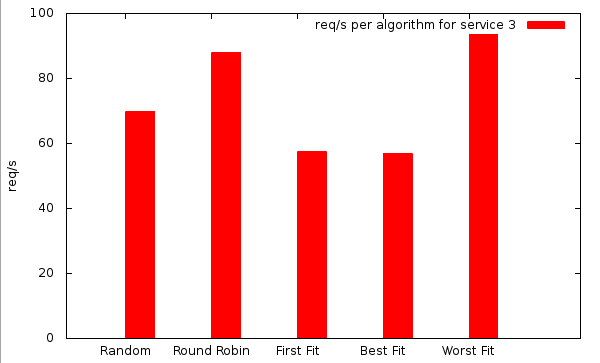
\includegraphics[width=\textwidth]{./Images/BinPacking/exp2-service3.png}
\label{fig:exp2service3}
\caption{Service 3: Number of requests per second for various algorithms}
\end{figure}

\vspace{1em}
\begin{tabular}{c | c | c | c}
	Algorithm & Number of used nodes & Performance rank \\
	Random & 7 & 3 \\
	Round-Robin & 7 & 2 \\
	First-Fit & 4 or 5 & 4 \\
	Best-Fit & 3 or 4 & 5 \\
	Worst-Fit & 7 & 1 \\
\end{tabular}
\captionof{table}{VMs allocation summary}
\vspace{1em}

\subsubsection{Results and discussions}

A first remark about those results is that, whatever is the service, and the
amount of requests it has to deal with, they behave the same way for each
algorithm. The graphs have the same shape with another ratio because some
container deal with much more queries.

Then, we can observe that as expected the best-fit and first-fit algorithms are
resulting to poorer performance. But what is shown in the allocation summary is
that those algorithms managed to use less virtual machines to pack all the
processes. They allocate resources on less than 5 of the 7 availables nodes.

Here is one of the biggest challenge, to get close to the highest performance
while using the minimum number of bins. There is direct solution for this problem
it really depends what is the main goal of the operation. If it is money saving,
reducing the number of virtual machines has a meaning, but the quality of service,
as the performance, should be high enough to respect the SLA\@.

Something which is more surprising is that an algorithm considered as
``intelligent'', which is worst fit, is only doing slightly better, and
sometimes even worse, than a simple algorithm like round robin.

The different *-fit algorithms need an estimation of the size of the incoming
item to pack. As stated previously, if the containers is part of an existing
service, the average of the usage of the other containers of this service will be
used. Otherwise, no estimation is done. This second condition seems to damage
those algorithm results.

To get over it, Some hybrid *-fit algorithms have been tried:

\begin{itemize}
	\item{Best-Worst Fit: This algorithm is using best-fit all the time except when
	the new item is from a new service, in this case, worst fit is used to pack
	it}
	\item{First-Worst Fit: Similar to best-worst fit but using first fit instead of 
	best-fit}
\end{itemize}

These variants should allocate more VMs than the base algorithms they are based on,
but they should be much more efficient for the same reason. As we have seen that the
results are mostly identical for the three differents services, we will focus on the
third one, it is not worthy to study the three of them.

\begin{figure}[h!]
	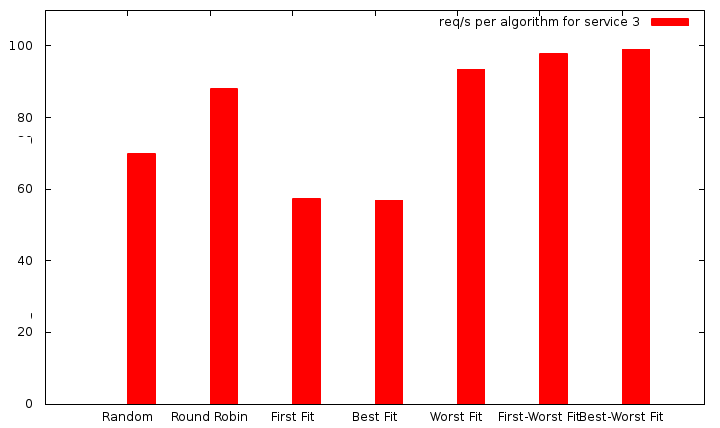
\includegraphics[width=\textwidth]{./Images/BinPacking/exp2ext-service3.png}
	\caption{Comparaison of *-fit algorithms performance}
\end{figure}

\vspace{1em}
\begin{tabular}{c | c | c | c}
	Algorithm & Number of used nodes & req/s for service 3 & Performance rank \\
	First-Worst Fit & 6 or 7 & 97.80 & 2 \\
	Best-Worst Fit & 5 or 6 & 99.05 & 1 \\
	Worst-Fit & 7 & 93.41 & 3 \\
\end{tabular}
\captionof{table}{Allocation summary with variants of *-fit algorithms}
\vspace{1em}

With these new results, we have successded to get slightly better results than
the standard worst-fit, and highly superior than the base algorithm each of the
variant is based on. First-Worst Fit and Best-Worst Fit are getting more or
less the same results but they are not using the same amount of nodes. From
that point, best-worst is clearly the best algorithm among them.  We could
alter those algorithms with some additional steps like sorting the bins before
starting the pack operation like it has been done
in~\cite{allocationHeterogeneous}.  However in this precise case it would be
without any effect. First-fit with ascending sorted bins result in Best-fit and
when the sort is descending it leads to Worst-fit, and we already know the
results of these methods.

We have seen that different methods exist, but to get a good ratio
performance/node usage, it may be required to mix the algorithms according to
the situation and the execution environment.  In our case, a mix of Best-fit
and Worst-fit has definitely got the most interessant results.

\subsection{Consolidation and load balancing --- offline bin packing algorithms}

\subsubsection{Impact on the infrastructure}

When an offline bin packing algorithm is applied on computing infrastructure,
to apply the new configuration, it results in a lot of migrations. When we are
dealing with full virtual machines, a migration has a cost and it is difficult
to imagine migrating several instances from one same host in parallel. With
containers, this issue doesn't exist and even less with stateless application

When a container has to be migrated, a new one is being started on the
destination server, then the routing table to the service is updated and
finally the source container is stopped. This operation can be done in less
than a second. Compared to VM migration which can last minutes and use a lot of
disk, network and CPU resources, the process which is used here costs almost
nothing.

If migrations were costly, caution should be taken when choosing the algorithm,
to avoid to do too many of them.

\subsubsection{Algorithms}

In this case, testing simple algorithms like round-robin or random would not be
interesting. They would result in the same data as what we have seen in the part
about online bin packing.

Offline bin packing algorithms are close to the online bin packing algorithm,
the differences are that we have all the pieces of information about the
running containers so there is no need to estimate any value. Then, there is
not only one item to pack anymore, but a list of items. An additional question
is in which order do the items have to be considered by the algorithms.
In~\cite{reassignmentElectricitysaving},~\cite{statisticalAssignment}
and~\cite{variableSizeBinPacking} they all refer to first-fit decreasing or
best-fit decreasing as reference algorithms. It means that the data are used
from the biggest to the smallest.

As a result 4 algorithms will be tested: Best-Fit Decreasing (BFD), First-Fit
Decreasing (FFD), the algorithm proposed by Michaël Gabay
in~\cite{variableSizeBinPacking} and the variant detailed
in~\cite{allocationHeterogeneous} where items are sorted decreasingly.

The used parameters are the following:

\begin{verbatim}
Gabay: heuristic=bin_balancing
Gabay: heuristic=bfd_item_centric
Gabay: heuristic=bfd_bin_centric
Stillwell: item_sort=d:maximal, pack=pack_by_items
\end{verbatim}

\subsubsection{Experiment}

The following experiment is based on the same services as the previous
experiment. This choice has been made because they have already been
benchmarked, and their range of performance is already known.  Refer to
the~\tref{tab:exp2-services}.

To obtain the data of the following graph, the underneath experiment has been done 5
times for each algorithm:

\begin{enumerate}
	\item{Start the load generation against the three services}
	\item{Deploy containers using a resource allocation algorithm which is not
	optimal. Best-fit has ben chosen because of the low result it has given in
	the previous experiment. This situation leads to overloaded nodes}
	\item{Run a first benchmark to get the performance before the offline bin
	packing algorithm execution}
	\item{Balance the infrastructure with the chosen algorithm}
	\item{Run a second benchmark to get the performance after the operation}
	\item{Calculate the average of the performance variation for the three services}
\end{enumerate}

Then once the previous protocol has been done 5 times, the average of the
result is the value displayed on the plot.\footnote{The detailed results for
the experiment can be found here:
\url{https://github.com/Soulou/msc-thesis-container-balancer-client/tree/master/experiment4}}

\begin{figure}[h!]
	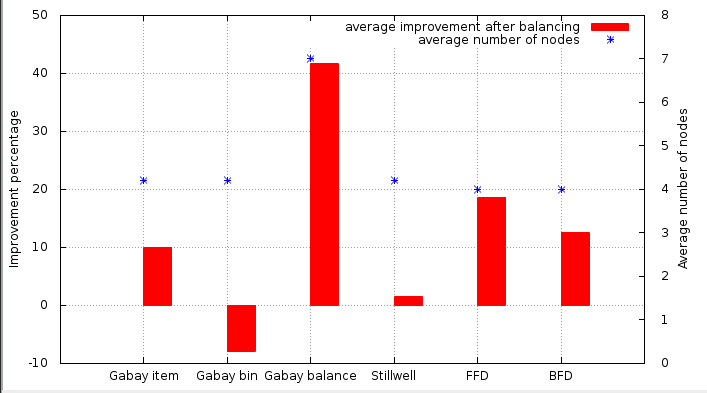
\includegraphics[width=\textwidth]{./Images/BinPacking/exp4_improvement.png}
	\caption{Performance improvement in function of the algorithm}
\end{figure}

\subsubsection{Results and Discussions}

The results are quite surprising. If \textit{Gabay balance} is shelved, the
different results are using the same amount of nodes, but their result are
unexpected.~\cite{allocationHeterogeneous} and~\cite{variableSizeBinPacking}
based their work on BFD and FFD, and build variations of them to fit specific
need, which is to work in an heterogeneous environment. Obviously it was not
the case here, but we could expect that those algorithms would have done at
least as good as BFD or FFD\@.

It is also possible that this error is due to a bad integration of the
algorithm in the container platform. Extensive testing would be required to
find if the behavior is buggy. It may be linked to how the data are normalized.
Everything is based on the bins. The server which as the highest capacity
results in the unit bin, with $1$ as capacity for each of his metrics, then all
the containers consumptions (items) and other bins are normalized using this
reference.  After this step, a reserve is subtracted from the capacity, to
avoid the algorithms to pack servers up to 100\% again. By default this reserve
is 20\%, and it seemd it suits well the implementations of BFD and FFD\@. But
Gabay's and Stillwell's algorithm are not working as they should. According to
their estimation in their work, they should both be more performant than BFD
and FFD\@.

The heuristic \textit{Gabay Balance} got great results which are really closed
to a simple worst fit allocation, all the nodes have been used and no effort
has been done to limit that. But, as a results, great performance is present.
If the goal of the operation is to balanced the load of the server, this approach
is probably the most efficient.

Comparing the two basics algorithms, FFD got slightly better results than BFD,
the difference is higher than the difference of those algorithms for online bin
packing, but the trend is similar. 

\vspace{1em}

Finally, the platform has proven that it is possible to get interesting metric
from it. In the previous experiments, containers have been deployed and
migrated with success resulting in performance variations. The three main
operation linked to resource allocation/re-assignment can be tested using this
infrastructure. If the online bin packing results are interesting, the data
collected for offline be packing are not resulting to a spcific recommandation.
 % Main experiments: algorithm testing
\chapter*{Conclusion}
\addcontentsline{toc}{chapter}{Conclusion}
\lhead{\emph{Conclusion}}

The purpose of this work has been to show how containers are a new efficient
way to isolate and deploy web applications. Then, we have seen that is it
possible apply limitation and quotas to limit how a container behaves. The next
step has been to design a software platform, aiming at deploying containers
easily into a cloud environment, but also to be able to move them between all
the available nodes. Furthermore this set of server appplications are gathering
real time metrics about the running containers and servers. With these data,
bin packing algorithms have been made possible and the last chapter of this
thesis has shown different experiments concerning the different way to use them
to allocate resource, consolidate the infrastructure or balance the load of the
servers.
\vspace{1em}

The developed platform has shown that it is able to manage efficiently
containerized web applications. This feature has lead to interesting results
concerning resource allocation. When a new container has to be run, we have
seen that a mix of simple bin packing heuristics is giving some really
interesting results. Combined together best fit and worst got the best ratio
``number of used nodes by number of answered requests per second''
\vspace{1em}

The field of resource allocation is getting more and more important now,
because infrastructure are getting more and more heavily distributed and I
have the feeling I have only scratched the surface of what can be done.
However, I think the developed platform is good enough and could extend
in order to be used for further experiments.
\vspace{1em}

This writing has principaly focused the obtained performance for containers
which were able to run without any limit. This is something which is really
common. A lot of service providers are based on a ``fair use'' policy. In this
case they do their best to run everything, but they can warn or give explicit
quota to user abusing this statement. If we get outside this scope, other
experiment should be done to get new results.
\vspace{1em}

Working in a real environment instead of a simulation changes a lot of settings,
I think that with the developed tools, a lot more testing and experiment
could be done, especially concerning load balancing. Another possible extension
could be some statistical prediction about the future consumption of a service,
based on statistical and probabilistical models. 
\vspace{1em}

A particular effort has been made to make this work reproducible. All the
tools are open-source softwares and protocols standard.  Thanks to
\textbf{Ansible} the environment should be easy to deploy on any
infrastructure, physical, virtual or hybrid.  Even if the obtained results in
another deployment of the platform would be slightly different, it should
follow the same trends as those obtained in this thesis.


%% ----------------------------------------------------------------
% Now begin the Appendices, including them as separate files

\addtocontents{toc}{\vspace{2em}} % Add a gap in the Contents, for aesthetics

\appendix % Cue to tell LaTeX that the following 'chapters' are Appendices

\lstset{xleftmargin=5pt}
% Appendix A

\chapter{Appendix Title Here}
\label{AppendixA}
\lhead{Appendix A. \emph{Appendix Title Here}}

Write your Appendix content here.% Agent API documentation

\chapter{HTTP API of the controller server}
\lstset{language=Javascript, basicstyle=\footnotesize\ttfamily}
\label{app:controller-api}

\vspace{1em}
\begin{lstlisting}

/*
 * Get the status of a given node, like the different resources consumption and total
 */
// GET /node/:host/status

// Code 404 - Agent not found

// Code 200 - OK
// Content-Type: application/json
{
  "cpus": {
    "cpu0": 44,
    "cpu1": 22,
  },
  "free_memory": 12300000,
  "memory": 27440000,
  "network": {
    "eth0": {
      "tx": 98765,
      "rx": 12345
    }
  }
}

/*
 * Return a list of containers running on a given host
 */
// GET /node/:host/containers

// Code 404 - Agent not found

// Code 200 - OK
// Content-Type: application/json
[
  {
    "Id": "0123456789abcdef",
    "Image": "soulou/msc-thesis-memory-http-service",
    "Ports": [
      {
        "PublicPort": 49127,
        "PrivatePort": 3000
      }
    ],
    "Names": [ "service1-1-837" ],
    "Created": 1723454345,
    "Status": "Up"
  },
  {
    ...
  }
]

/*
 * Return the status of all the nodes of the cluster.
 */
// GET /nodes/status

// Code 200 - OK
// Content-Type: application/json
{
  "192.169.0.1" : {
    "cpus": {
      "cpu0": 44,
      "cpu1": 22,
    },
    "memory": 27440000,
    "network": {
      "eth0": {
        "tx": 98765,
        "rx": 12345
      }
    }
  },
  "192.168.0.2" : ...
}

/*
 * This endpoint aims at executing an algorithm of load balancing.
 * The name of the algorithm has to be given in the strategy parameter
 * The containers and the agents nodes resource usage is gathered then normalized,
 * then the algorithm is executed.
 * As a result of the problem solving, a set of migration is applied to move
 * the containers according to the algorithm solution.
 */
// POST /balance
// Params:
//   strategy: "stillwell_current"

// Code 200 - OK
{
  "items": [[0.2, 0.3, 0], [...]],
  "bins": [[1.0, 2.0, 1.0], [...]],
  "problem": {
    "algo": "stillwell_current",
    "mapping": [0,0,0,1,2,3,4],
  },
  "migrations": [
    {
      "Service": "service-1",
      "Started": {
        "host": "182.168.0.2",
        "id": "0123456789abcdef"
      },
      "Stopped": {
        "host": "182.168.0.2",
        "id": "0123456789abcdef"
      }
    },
    {
    ...
    }
  ]
}

// GET /containers

// Code: 200 - OK
// Content-Type: application/json
[
  {
    "Host": "192.168.1.2",
    "Id": "0123456789abcdef",
    "Image": "soulou/msc-thesis-memory-http-service",
    "Ports": [
      {
        "PublicPort": 49127,
        "PrivatePort": 3000
      }
    ],
    "Names": [ "service1-1-837" ],
    "Created": 1723454345,
    "Status": "Up"
  },
  {
    ...
  }
]

// POST /containers

// Code: 201 - Container started

// Docker JSON representation of a container:
// With an additional field: "Host"
// See: http://goo.gl/JrR6f6


// DELETE /container/:host/:container_id

// Code: 404 - Host or Container not found
// Code: 204 - Container stopped


// POST /container/:host/:container_id/migrate

// Code 200 - Container migrated
{
  "Service": "service-1",
  "Started": {
    "host": "182.168.0.2",
    "id": "0123456789abcdef"
  },
  "Stopped": {
    "host": "182.168.0.2",
    "id": "0123456789abcdef"
  }
},

\end{lstlisting}
 % Controller API documentation

\chapter{Client command line tool documentation}
\lstset{language=Bash, basicstyle=\footnotesize\ttfamily}
\label{app:client-doc}

\vspace{1em}

\begin{itemize}
\item{Start a container
\begin{lstlisting}
./client.py start [--image <image name>] <service name>

##
# The Image parameter correspond to the docker image which should be
# run on the agent, as at that time, the identify of this agent is not
# known, take care that all the agents have the requested docker image.
# By default a fibonacci web service is executed.
#
# The service name is the name of the group of containers that the
# newly created process will be appended, if the group doesn't exist,
# it is created.
#
# Example
#

./client.py start --image soulou/memory-http-service service1

-> Host: 192.168.114.13
-> ID: e6bbb8853678b67882ea6919c559d80a20
-> Service: service1
-> Image: soulou/msc-thesis-memory-http-service
-> Port: 49342
\end{lstlisting}}
\item{Stop a container
\begin{lstlisting}
./client.py stop --service <service_name> | --all <host> | <host> <ID>

##
# Three different options are available to stop a container.
# * All the container of a service ban be stopped
# * All the container of a precise server may be stopped
# * A precise container can be shutdown by giving its host and its ID
#
# Example
#

./client.py stop --service <service_name>

Container f6fe748fbf from 192.168.114.14 has been stopped
Container e7dc0f68f3 from 192.168.114.17 has been stopped
Container 6a28e4b2ab from 192.168.114.15 has been stopped
\end{lstlisting}}
\item{Get status of the infrastructure
\begin{lstlisting}
./client.py status

##
# Give the information about all the running containers
#
# Output example
#

+----------------+-------+-----------+
| Node           |  Port |  Service  |
+----------------+-------+-----------+
| 192.168.114.14 | 49196 |  service3 |
| 192.168.114.14 | 49195 |  service3 |
| 192.168.114.13 | 49342 |  service1 |
+----------------+-------+-----------+

+---------------------------------------+
|                 Image                 |
+---------------------------------------+
| soulou/msc-thesis-memory-http-service |
| soulou/msc-thesis-memory-http-service |
| soulou/msc-thesis-memory-http-service |
+---------------------------------------+

+-----------------+---------------------+
|        ID       |      Created At     |
+-----------------+---------------------+
| 3c9345c19e00d21 | 2014-07-28 10:51:34 |
| 9a2e2b22448f766 | 2014-07-28 10:51:33 |
| e6bbb8853678b67 | 2014-07-29 15:52:15 |
+-----------------+---------------------+
\end{lstlisting}}
\item{Migrate an application to another node
\begin{lstlisting}
./client.py migrate <host> <id>

##
# This operation asks the controller to migrate a container
# to another node
#
# Example
#

./client.py migrate 192.168.1.3

Container 192.168.1.3 - 9a2e2b2244 -> 192.168.1.18 - 406d5ce46d
\end{lstlisting}}
\item{Load balance infrastructure
\begin{lstlisting}
./client.py balance [--opt opt1=val1 [--opt opt2=va2 ...]] <algorithm>

##
# Run a load balancing or consolidation
# operation on the complete infrastructure
# The algorithm can be specified the following
# are available:
#
# Implemented in the controller
# [first-fit-decreasing, best-fit-decreasing]
#
# Implemented in third-party library
# [stillwell, gabay2013vsvu, brandao2013mvp]
# https://github.com/marklee77/vpack
#
# Example
#

./client.py balance \
  --opt heuristic=bin_centric \
  --opt bin_measure=do_nothing \
  --opt item_measure=do_nothing \
  gabay2014vsvu

{'bins': [{'capacity': [0.8, 0.8, 0.8],
	  'remaining_capacity': [1.0, 1.0, 1.0]}, ...],
 'items': [[0.0, 0.0004, 0.0], ...]
 'migrations': [{'Service': 'service2',
                 'Started': {'Id': '7724621e2dcccb472',
                             'Node': '192.168.114.14'},
                 'Stopped': {'Id': 'd3f8a1e45481e3945',
		 'Node': '192.168.114.13'}}, ...],
 'result': {'algo-runtime': 0.00013580999999973642,
            'bincount': 7,
            'datetime': '2014-08-10 18:04:28.343690',
            'failcount': 0,
            'family': 'gabay2013vsv',
            'kwargs': {'bin_measure': 'do_nothing',
                       'family': 'gabay2013vsv',
                       'heuristic': 'bin_balancing',
                       'item_measure': 'do_nothing'},
            'mapping': [0, 1, 2, 3, 4, 5, 6, 0, 1, 2],
            'problem-argshash': None,
            'solver-githash': '__GITHASH__',
            'total-runtime': 0.00021365099999925974,
            'verified': True}
}

\end{lstlisting}
}
\item{Get node or nodes status
\begin{lstlisting}
./client.py node_status <host>
./client.py nodes_status

##
# Get the system metrics for on particular node or all the nodes
#

./client.py nodes_status
[ '192.168.114.19': {'cpus': {'cpu0': 0, 'cpu1': 0},
                    'free_memory': 3736440,
                    'memory': 4048292,
                    'nb_containers': 0,
                    'net': {'docker0': {'rx': 0, 'tx': 0},
                            'eth0': {'rx': 3728, 'tx': 1858},
                            'eth1': {'rx': 0, 'tx': 0},
                            'lo': {'rx': 0, 'tx': 0},
                            'veth2074': {'rx': 0, 'tx': 0},
                            'vetha4f2': {'rx': 913, 'tx': 1796},
                            'vethc390': {'rx': 0, 'tx': 0},
                            'vethd466': {'rx': 633, 'tx': 964},
                            'vethec34': {'rx': 0, 'tx': 0}}}}
]
\end{lstlisting}}
\end{itemize}
 % Client Documentation
\chapter{Projects related to the thesis}
\label{app:rel-projects}

\begin{itemize}
\item{\url{https://github.com/Soulou/msc-thesis-container-balancer-agent}

The repository contains the code of the agent, which is running on every
hosting server, monitoring the host and its container in real time.}

\item{\url{https://github.com/Soulou/msc-thesis-container-balancer-controller}

The controller of the infrastructure which finds the agents through
\textbf{Consul}. It manages the allocation and the load balancing operations in
the infrastructure.}

\item{\url{https://github.com/Soulou/msc-thesis-container-balancer-client}

The client is a simple CLI tool to communicate with the controller. Otherwise
it would be necessary to write the HTTP requests by hand, which is not really
confortable.}

\item{\url{https://github.com/Soulou/msc-thesis-fibo-http-service}

Webservice generating numbers of the fibonacci sequence. Used as a docker image
to generate load.}

\item{\url{https://github.com/Soulou/msc-thesis-memory-http-service}

Webservice allocating a precise amount of memory during a precise duration,
used to simulate different kinds of webservices}

\item{\url{https://github.com/Soulou/msc-thesis-cpu-burn}

Small software design to use completely a given amount of CPU cores.}

\item{\url{https://github.com/Soulou/msc-thesis-container-cpu-monitor}

Tool to generate data about the consumption of each container run by
\textbf{Docker}.}

\item{\url{https://github.com/Soulou/msc-thesis-cloud-builder}

Set of tools designed to deploy VMs automatically in an \textbf{OpenStack}
environment.}

\item{\url{https://github.com/Soulou/msc-thesis-ansible}

\textbf{Ansible playbook to deploy everything required to run the exeperiment
on the VMs dpeloyed by the Cloud Builder.}}
\end{itemize}
 % List of projects

\addtocontents{toc}{\vspace{2em}}  % Add a gap in the Contents, for aesthetics
\backmatter

%% ----------------------------------------------------------------
\label{Bibliography}
\lhead{\emph{Bibliography}}  % Change the left side page header to "Bibliography"
\nocite{*}
\bibliographystyle{unsrtnat}
\bibliography{Bibliography}

\end{document}  % The End
%% ----------------------------------------------------------------
